\documentclass[12pt]{article}

%% preamble: Keep it clean; only include those you need
\usepackage{amsmath}
\usepackage[margin = 1in]{geometry}
\usepackage{graphicx}
\usepackage{booktabs}
\usepackage{natbib}
\usepackage[T1]{fontenc}


% for space filling
\usepackage{lipsum}
% highlighting hyper links
\usepackage[colorlinks=true, citecolor=blue]{hyperref}

\usepackage{float}
\usepackage{setspace}



%% meta data

\title{Analyzing Player Performance in Premier League Soccer Using 
Data Visualization and Predictive Analysis}
\author{Okem Chime\\
  University of Connecticut
}

\doublespacing
\begin{document}
\maketitle

\begin{abstract}

In the realm of predictive modeling for player performance in Premier League
soccer, this research endeavors to explore the influence of historical data on
goal contributions per 90 minutes. Utilizing a dataset encompassing key
performance metrics, including age, position, and minutes played, we investigate
the predictive capabilities of various machine learning models. The evaluation
metrics employed, such as Mean Squared Error (MSE), Mean Absolute Error (MAE),
and Correlation, offer a comprehensive assessment of model performance.

Six distinct models, including Decision Tree, Gradient Boost, Kernel Ridge,
Linear Regression, Random Forest, and Ridge Regression, were compared. Notably,
Gradient Boost emerged as the optimal model with the lowest average MSE (0.041)
and MAE (0.150). Our findings reveal that historical player performance data,
coupled with relevant variables, serves as a robust foundation for accurate
predictions of future goal contributions. This aligns with the broader context
of predictive modeling in sports, echoing the efficacy of such approaches
demonstrated in prior studies.

\end{abstract}


\section{Introduction}
\label{sec:intro}


%The introduction is used to a refernce framework for the reader. 
%The aim of this section is to answer three questions:
%Why is the topic important/interesting?
%What has been done on this topic in the literature?
%What is your contribution?


For many people worldwide, sports transcend the realms of mere games or leisure
activities, acting as a unifying force that transcends geographical, linguistic,
and cultural boundaries. Global sporting events, exemplified by the Olympic Games
and the World Cup, underscore the profound significance of sports in fostering
global unity. Beyond its cultural impact, the sports industry wields substantial
financial power, exerting significant economic and social influences. It serves
as a catalyst for revenue generation, tourism influx, and job opportunities,
playing a pivotal role in the economies of many nations.

Within the vast landscape of data science, sports performance data represents a
burgeoning and expansive field. The intricate details of professional sports
provide a fertile ground for data science techniques, offering a potential
competitive edge to players and teams. Soccer, being the world's most popular
sport with over 3.5 billion fans globally and more than 250 million players
across 200 countries, stands as a prime arena for data-driven insights.

At the epicenter of this global passion for soccer is the English Premier League,
a sports spectacle watched by millions worldwide, boasting a potential viewership
exceeding 4.7 billion individuals. The league's immense popularity makes it a
critical focal point for players, coaches, fans, sponsors, and stakeholders alike.
The success of both the league as a whole and the individual performances of teams
and players significantly impacts various facets of the sport.

In this high-stakes environment, data science emerges as a game-changer through
sports performance analysis. This domain revolutionizes the sporting landscape
by introducing a new layer of insights that were once unimaginable. The
statistical revelations derived from data science have the potential to guide
decisions at all levels of the game- from players on the pitch to the fans in
the stadium. By delving into the intricacies of player performance, tactics, and
team dynamics, sports performance analysis transforms raw data into actionable
intelligence, offering a nuanced understanding of the game that goes beyond
traditional observations.


%% lit review p1:
Recent studies, such as the work by \citet{goes2021unlocking} have underscored
the growing significance of big data in professional soccer, particularly with
the widespread adoption of wearable position tracking devices. These technological
advancements offer a wealth of data that has been recognized as a potential
game-changer in high-performance sports. 

This paper's aim was to assess the contributions of both sports science and
computer science to the analysis of tactical behavior in soccer using position
tracking data. Their objective was to provide a thorough evaluation of the
methodologies employed in relevant studies from both domains, identify
differences, and propose a framework for optimizing collaboration between sports
science and computer science to enhance the analysis of tactical behavior in soccer.

The methodology involved a systematic review of studies from both sports science
and computer science that utilized position tracking data for analyzing tactical
behavior in soccer. The paper critically examined the research questions,
problem definitions, data collection methods, spatial and temporal aggregation
techniques, as well as the modeling and interpretation approaches employed in the
selected studies.

Key findings from the review revealed substantial differences in the research
paradigms of sports science and computer science. Sports science studies primarily
focused on deductive reasoning, theoretical frameworks, and experimental designs
aimed at advancing the understanding of tactical behavior and its practical
implications. On the other hand, computer science contributions were characterized
by inductive reasoning, data-driven methodologies, and a focus on developing new
computational techniques rather than emphasizing practical implications.

The paper identified a spectrum in the collaboration between the two domains,
showcasing studies that gravitate toward the sports science end, the computer
science end, and those in the middle that exemplify the synergy between both.
They emphasized the potential benefits of a cyclical collaboration, where sports
science informs theory and practical problems, and computer science contributes
tools and methodologies to enhance the analysis of tactical behavior.

Our work contributes to the evolving discourse initiated by \citet{goes2021unlocking},
expanding the scope beyond tactical considerations and delving into how performance
data can serve as a comprehensive guide for decision-making in the realm of
player analysis and management. The cyclical collaboration framework proposed in
the systematic review aligns with our goal of integrating expertise from both
domains, ultimately enhancing the depth and applicability of our research findings.

However, while \citet{goes2021unlocking} primarily delved into the tactical
implications of this position tracking data, our research focuses on the  
utility of performance data as related to player performance. 
Our study recognizes the potential of this data to guide decision-making about
indivdual players from a performance evalutation perspective- rather from the 
wider tactical lens associated with overall team performance.


%% new lit rev part 2
Some interesting work was done by \citet{tunaru2010valuations} where
the authors aimed to develop a statistical model for
determining the financial value of soccer players based on their past performance.
The methodology involved utilizing the OPTA Index, a database with over 400
variables recorded for all games in the English Premier League. This index
encapsulates the individual performance of players and teams, allowing for
relative value calculations and methodologies for financial valuation of players
and clubs.

The key findings of the paper included demonstrating how statistical analysis of
past performance, as represented by the OPTA Index, could be instrumental in
assessing the financial value of soccer players. The authors illustrated this by
examining the case of Thierry Henry during the EPL season 2003-04, highlighting
the correlation between his individual performance and the financial value
attributed to him by his club. The paper also discussed the vulnerability of
players as assets, emphasizing the differences in financial value when viewed
from the perspective of the current and potential new clubs.

Drawing parallels between their work and mine, both studies leverage OPTA data
as a foundational element for evaluating player performance. However, the key
distinction lies in the scope of factors considered. Tunaru and Viney incorporate
both on-field and off-field metrics to inform their financial evaluations,
whereas my research, aligning with the scope of my thesis, centers on objective
on-field performance data. This deliberate focus aims to unravel insights into
players' current performance levels and offers predictions regarding their future
on-field contributions.


%% lit review part 3
Another intreesting study was conducted by \citet{geurkink2021machine} who used
a machine learning model to obtain the most important factors in winning and
losing using data from the Belgian Profesisonal Soccer league to 
predict whether a specific match would be won or lost.

The researchers constructed a predictive
model drawing upon a comprehensive dataset of 576 games and a multitude of
variables (n = 100). To refine their model, techniques like Variance Inflation
Factor (with a threshold of 5) and BorutaShap were enlisted to mitigate
multicollinearity and manage dimensionality. From the exhaustive set of variables,
a discerning 13 were retained for forecasting wins or losses, utilizing the power of
Extreme Gradient Boosting.

In dissecting the model's insights, the study attained an impressive accuracy of
89.6\% ± 3.1\%, with notable precision (88.9\%), recall (90.1\%), and f1-score
(89.5\%). This translated to the correct classification of 516 out of the 576
games analyzed. Intriguingly, the variable "shots on target from the attacking
penalty box" emerged as the standout predictor. Beyond this, the study shed
light on the significance of various physical indicators and contextual
variables, including ELO ratings, the added transfer value of benched players,
and even the location of the match.

These findings underscore the added value derived from incorporating a diverse
array of variables when forecasting and evaluating soccer game outcomes. The
study advocates for similar modeling approaches to be adopted by soccer clubs,
offering a pathway to identify pivotal predictive variables tailored to their
leagues. Consequently, this approach not only aids in predicting match results
but also empowers clubs to enhance their current quantitative analyses for
strategic decision-making.

This study draws a lot of parallels with our research as their study employs
a predictive component within soccer; they draw on in game statisitcs as variables
in their model in a similar manner to this paper. Where their research differs
is their focus is on in game statistics based around the entire team
whereas the variables drawn upon in this study are performance metrics based on 
an individual player. This study also attempts to make predictions about whether
a team will win a specific game as well as identify the most important factors
involved in this process however, in this paper our predicitons occur on the
level of the player as opposed to the team and doesn't attempt to identify
any outstanding variables in terms of their importance in predicting player 
performance within our model.

% lit rev pt 4

Some work was done where basketball was the focus of the study. 
The study in question aimed to delve into the structural intricacies of shooting
performances among elite basketball players during FIBA EuroBasket 2015.
The analysis centered on dissecting the execution of shots concerning footwork
(one- or two-count stop, etc.) and handwork (one-hand overhead, layup, floater, etc.). 
Beyond this, the study harbored a secondary objective: to compare the shooting
performance between the top eight teams (Places 1–8) and the bottom eight teams
(Places 17–24) participating in the event \citep{gryko2018structural}.

A comprehensive examination was conducted, covering 9024 shots across all matches
(n = 110) played by the top eight teams (n = 70) and the teams eliminated in the
early stages (n = 40). The methodology adopted a categorized observation approach,
with subsequent data analysis relying on ANOVA (post hoc Tukey’s test) and a
multiple ridge regression.

The outcomes of the study, as revealed by the regression analysis and reference
values, unveiled intriguing insights. For the top-performing teams, the number of
successful two-point shots emerged as the paramount predictor of the points scored
(F = 35.51, p = 0.001). Conversely, for the lower-ranked teams, the pivotal
predictor for points scored was identified as the number of successful
three-point shots (F = 21.82, p = 0.001). This nuanced analysis not only
contributes to a deeper understanding of shooting structures in elite basketball
but also provides valuable insights for strategic considerations in team
performance \citep{gryko2018structural}.

Although this study exists in a different sporting context to that of this paper,
a common thread is shared in their analytical approach toward performance outcomes.
While the study done by \citet{gryko2018structural}
investigates shooting structures and predictors of success, our soccer-oriented
research focuses on the predictive modeling of player performance based on
historical data.

Both studies employ statistical analyses to derive meaningful insights.
The \citet{gryko2018structural} study uses ANOVA and multiple ridge regression.
We see similarity in that our study also utilises ridge regression and other
regrression technqiues such as linear regression. However, in our research we also 
leverages machine learning techniques such as  Gradient Boosting, Random Forest
and Decision Trees.

We also acknowledge that both studies recognize the significance of various
variables in influencing outcomes.
The \citet{gryko2018structural} study identifies the importance of successful
two-point and three-point shots, whilst our soccer research incorporates a broad
spectrum of player-related variables (e.g., goals, minutes played, assists) for
predictive modeling.


% lit review part 5

The investigation conducted by \citet{russell2013technical} delves into
the intricate relationship between match play and the technical performance of
professional soccer players, with a specific focus on outfield players within the
English Championship during the 2010/2011 season. Employing computerized
notational analysis, the study retrospectively evaluated the temporal patterns
in the performance of ten outfield players who participated in more than 10 games.

The primary aim of the study was to discern the impact of match-specific factors
on various technical aspects of player performance. The analysis considered key
variables, including total possessions and the number of ball distributions. The
temporal dimension was a crucial aspect, with a detailed examination of
performance across halves and specific 15-minute intervals within each game.

The findings of the study revealed noteworthy trends. In the second half of match
play, there was a substantial reduction of 10\% in total possessions and an 11\%
decrease in the number of ball distributions compared to the first half.
Moreover, a nuanced analysis across 15-minute intervals unveiled a decline in
both total possessions and distributions during the concluding 15 minutes of the
match.

However, amidst these reductions, certain technical metrics remained consistent.
Touches per possession, the number of challenges, challenge success rates, the
length of forward distributions, and the success rates of distributions exhibited
stability between halves and across 15-minute intervals.

The implications of these findings extend to the realm of coaching and team
management. Understanding that match-specific dynamics influence the total
possessions and ball distributions in the second half of soccer matches provides
coaches with valuable insights. This information can be utilized to tailor team
tactics and enhance technical training sessions, ultimately optimizing player
performance.

While my study can also contributes to the understanding of player performance,
it approaches this from a different lens. While the study by
\citet{russell2013technical} primarily deals with the impact of match-specific
factors on technical metrics during the course of a single match, my research is
oriented towards a broader predictive scope, attempting to discern patterns and
formulate predictions for an entire season based on historical data. 
The methodology shifts from retrospective notational analysis to a
forward-looking approach, utilizing machine learning techniques and leveraging
data from previous seasons to construct a model capable of forecasting a
player's offensive contributions.


% lit review part 6

A study that also used predictive modelling in their research was conducted by
\citet{blanchfield2019developing} which delved into the development of predictive
models for athletic performance, emphasizing the creation of informative decision
support tools for coaches and trainers.
The study aimed to utilize biometric data to predict athletic performance and
inform training regimens and in-game strategies.

The study utilized data collected by the University of Virginia's varsity field
hockey team, incorporating a range of sources.
Biometric data was captured during practices and games using Polar monitors,
providing insights into player performance.

A proprietary data frame was constructed, combining biometric features derived 
from 10Hz Polar data streams (e.g., heart rate, distance, velocity, acceleration,
cadence, GPS, R-R intervals) for each player.

The study revealed that the intensity of training sessions leading up to a
competitive match significantly influenced the game's outcome, whether it
resulted in a win or a loss.
Specifically, it found that high cardiovascular training loads two days before a 
competition were predictive of a victory.
Additionally, statistically significant differences were identified in the
physiological behaviors of players in different positions; the implications of
understanding these positional differences has the ability to guide
position-specific training and strategies.

This study demonstrated the potential for predictive models to inform coaching
decisions and player development as well as highlighting the significance of
considering multiple performance metrics and the timing of training sessions for
improved outcomes in team sports.

Although this study exists within a different sporting context to that of this 
paper, paralles can be found in how it uses performance data and predictive
modelling to inform decisions. However, their research uses biometric data from 
athletes in their research whereas the performance data used in our investigation
uses data that can be captured in a notational fashion- such as goals, assists 
etc. Our study also differes in the fact that our study looks at the ability
of our predictive model to forecast player performance over a whole season using
historical data as opposed to predicting the outcome of a singular match.



% objectives/ specific aims - tweak
The objective of this paper will be to investigate how data visualization and
predictive analysis can be used to assess and improve player performance in
Premier League soccer. It then seeks to answer the quesion:
"How does historical player performance data, including key performance
metrics influence the prediction of player's goal contributions
(combined goals and assists) per 90 minutes in future Premier League 
soccer matches, and how can this information be leveraged for strategic 
decision-making?".

By analyzing the performance statistics of premier league 
players from previous years, this paper will able to decipher the important
factors that are significant in contributing to a player's total goal
contributions per 90 minutes in a premier league season. From this, we will use 
statistical techniques to build a model which can predict a player's goal 
contributions per 90 minutes for a specific premier league season on the basis
of their previous performance history. 

This study will focus on a subset of 9 
midfield and attacking players who have competed in all 10 of the most recent 
premier league seasons. Goal contributions are an important metric within soccer
because of the simple fact that goals are the single factor which determines
which team will win a soccer match. Assists are also highly valued as they are
the vital previous step which leads to a goal and are thus an important metric
in attacking play.

Due to the fact that attacking players
play further up the field they are expected to primarily contribute goals to the 
team, as well as some assists.
Midfielders are expected to cover all areas of the field, thus due to having
more defensive responsibilites than attackers, while still expected to
contribute some amount of goals, due to their role in connected defence to
attack are expected to primarily provide assists. 

Thus, the metric of combined goals and assists (known as 'goal contributions') is 
a very good statisitc to measure a player's overall attacking productivity.
By including a player's assists it somewhat removes the bias of attacking players
to achieve better attacking productivity due to their advantage of them playing 
much higher up the field- although not completely. Goals contributions per 90 
minutes is the performance metric primarily focused on this paper because it
aids in removing the bias achieved from a player having played a greater amount 
of minutes than another, due to the fadct that the more minutes you play, the
more opportunity you have to score or assist a goal.



% roadmap
The rest of the paper is organized as follows.
The data will be presented in Section~\ref{sec:data}.
The methods are described in Section~\ref{sec:meth}.
The results are reported in Section~\ref{sec:resu}.
A discussion concludes in Section~\ref{sec:disc}.


\section{Data}
\label{sec:data}


% Utilize this segment to provide an account of the data essential for addressing
% your research inquiries. 

In this study, the primary source of data is the Premier League OPTA performance
data obtained from the reputable and comprehensive website, Fbref.com.
Fbref.com provides detailed player and team statistics for various soccer
leagues, including the Premier League, making it a reliable foundation for our
research.

The dataset encompasses a wide range of metrics that collectively form a
comprehensive overview of a player's on-field performance. These metrics include
fundamental statistics such as matches played, goals scored, and assists.
Additionally, the dataset incorporates more intricate metrics like expected goals
and assists, which offer valuable insights into the nuanced aspects of player
performance.

To ensure a robust and extensive analysis, we will be utilizing data spanning
ten seasons, from the 2013-14 Premier League season to the 2022-23 season.
This decade-long timeframe enables us to capture a substantial sample of player
performances, allowing for a thorough examination of trends and patterns over
the years. Using 10 seasons of performaance data also provides a quantity of 
data extensive enough to draw reliable insights from as well as provide enough
data input to use for our models for the predictive portion of the research.
On average each competitive season provides approximately 530 observations-
representing the number of players that competeted in that Premier League 
season. For each observation, the data from seasons 2013-14 until 2016-17 contain
23 variables whilst from seasons 2017-18 until 2022-23 contains 35 variables.
The additional variables represented in the more recent Premier League seasons
represents the performance metrics associated with 'expected goals', which was
not a commonly adopted performance statistic in earlier Premier League seasons.





\section{Methods}
\label{sec:meth}


% Utilize this section to introduce the methodologies that will produce results 
% through the analysis of the provided data.

% data collection
This research commenced through collecting the performance data. Using 
Fbref.com as our data source we were able to download 10 seasons of player
performance data into microsoft excel where we could better manipulate and 
analysze the data. 
% data cleaning
The data then had to be cleaned make it usable via deleting uneeded cells which
didn't provide statistical data as well as other pieces of miscellaneous text 
which had been imported during the downloading process. 
% importing to python + operations on the data
From here we imported these excel sheets into python- which will be the 
statistical software of choice for the research project. Using pandas enabled
us to create 10 seperate python files for each season of Premier League data and 
store them as a dataframe. One issue that was indentified in the data was that 
if a player had switched teams during the middle of the season their name would 
appear twice in the dataset. To remedy this, we created a python script which 
itreated through each dataframe and checked if a player's name appeared more 
than once in a dataset- if the player's name appeared only once then their attributes
would get immediately added to the dataframe however, if their name appeared twice
then we would have to aggregate their data into a single entry- for example,
summing together attributes such as goals, assists and minutes played and then 
adding them to the dataframe.

Next, we had to amalgamate all this data together. The idea was to create a 
large dataframe composed of the 10 dataframes containing performance data for players 
in each Premier League season. This required importing all of these dataframes 
into a central python file. We then extracted all the unique player names from
all the seasons by adding each player name to a set then converting it to a list.
This resulted in a total of 1895 unique players who had featured in the Premier
League across all 10 seasons.

Now that we had identified every unique player, our aim was to create 10 new 
dataframes containing all 1895 players for each season. By importing the unique
player names list into a python script coresponding to each season, we imported 
the dataframe corresponding to that specific season and for each name in the 
unique player names list we checked if the current player featured in that specific 
season by checking if they appeared in the dataframe. If they did feature in that 
speciifc season they would get added to the dataframe immediately whereas if a 
player didn't feature they would get added to the dataframe with 'NaN' values 
as their attributes. 

We were then able to create a 3 dimensional tensor- consisting of the dimensions 
player name, season and player attributes for each season- from these 10 dataframes
by concatinating them all into this central tensor. 
We then iterated through the tensor to find the players who had featured in all 
10 seasons and added them to a list. From this list we were able to identify 
9 forward/midfield players upon which to base our research upon. These players 
include:
Harry Kane, Raheem Sterling, Wilfried Zaha,
James Ward-Prowse, Jordan Henderson, Danny Welbeck,
Adam Lallana, Alex Oxlade-Chamberlain and Theo Walcott.

At this point we were then able to conduct the predictive portion of our research.
The idea was to implement a 'rolling-window' approach to training our model. 
We would train the model by inputting the players 'G+A/90' (Goals + Assists per 
90 minutes) for the previous 3 seasons as well as their position position, age 
and minutes played for the current season that we would be trying to predict.
This would then be compared to the player's actual 'G+A/90' value for the season
and then the model would continue on in this fashion- sliding the window 
forward one season at a time unitl it provided a prediction 
for the final season.
This meant that for each player the model would provide 6 predictions, starting
from the 4th season (2016-17) up until the final season (2022-23). This approach 
allowed us to train the model on a dynamic dataset as we moved through the seasons.

We then applied different models to our research to assess which one performed 
the best in comparison to the actual 'G+A/90' values for each player. We chose 
6 different modelling techniques:
Linear Regression, Decision Tree, Random Forest, Gradient Boosting, Kernel Ridge 
and Ridge Regression.
We evaulated the results by calculating the 
Mean Squared Error (MSE), Mean Absolute Error (MAE) and Correlation (Corr) for 
each player's set of predictions as well as calculating the average MSE, MAE and 
Corr across all 9 players for each model in order to compare each model's 
overall performance against one another.
After selecting the best performing model, we then displayed the prediction
results for each of the 9 players players using this model.





\section{Results}
\label{sec:resu}

% table comparing model performance


\begin{table}[H]
  \centering
  \begin{tabular}{|l|c|c|c|}
  \hline
  \textbf{Model} & \textbf{Average MSE} & \textbf{Average MAE} & \textbf{Average Correlation} \\
  \hline
  Decision Tree & 0.045 & 0.157 & -0.001 \\
  Gradient Boost & 0.041 & 0.150 & -0.110 \\
  Kernel Ridge & 0.168 & 0.331 & 0.163 \\
  Linear Regression & 2.927 & 0.597 & -0.252 \\
  Random Forest & 0.042 & 0.153 & -0.324 \\
  Ridge Regression & 0.080 & 0.214 & -0.316 \\
  \hline
  \end{tabular}
  \caption{Model Performance Comparison}
  \label{tab:model_performance}
  \end{table}


  % zaha figure

\begin{figure}[H]
  \centering
  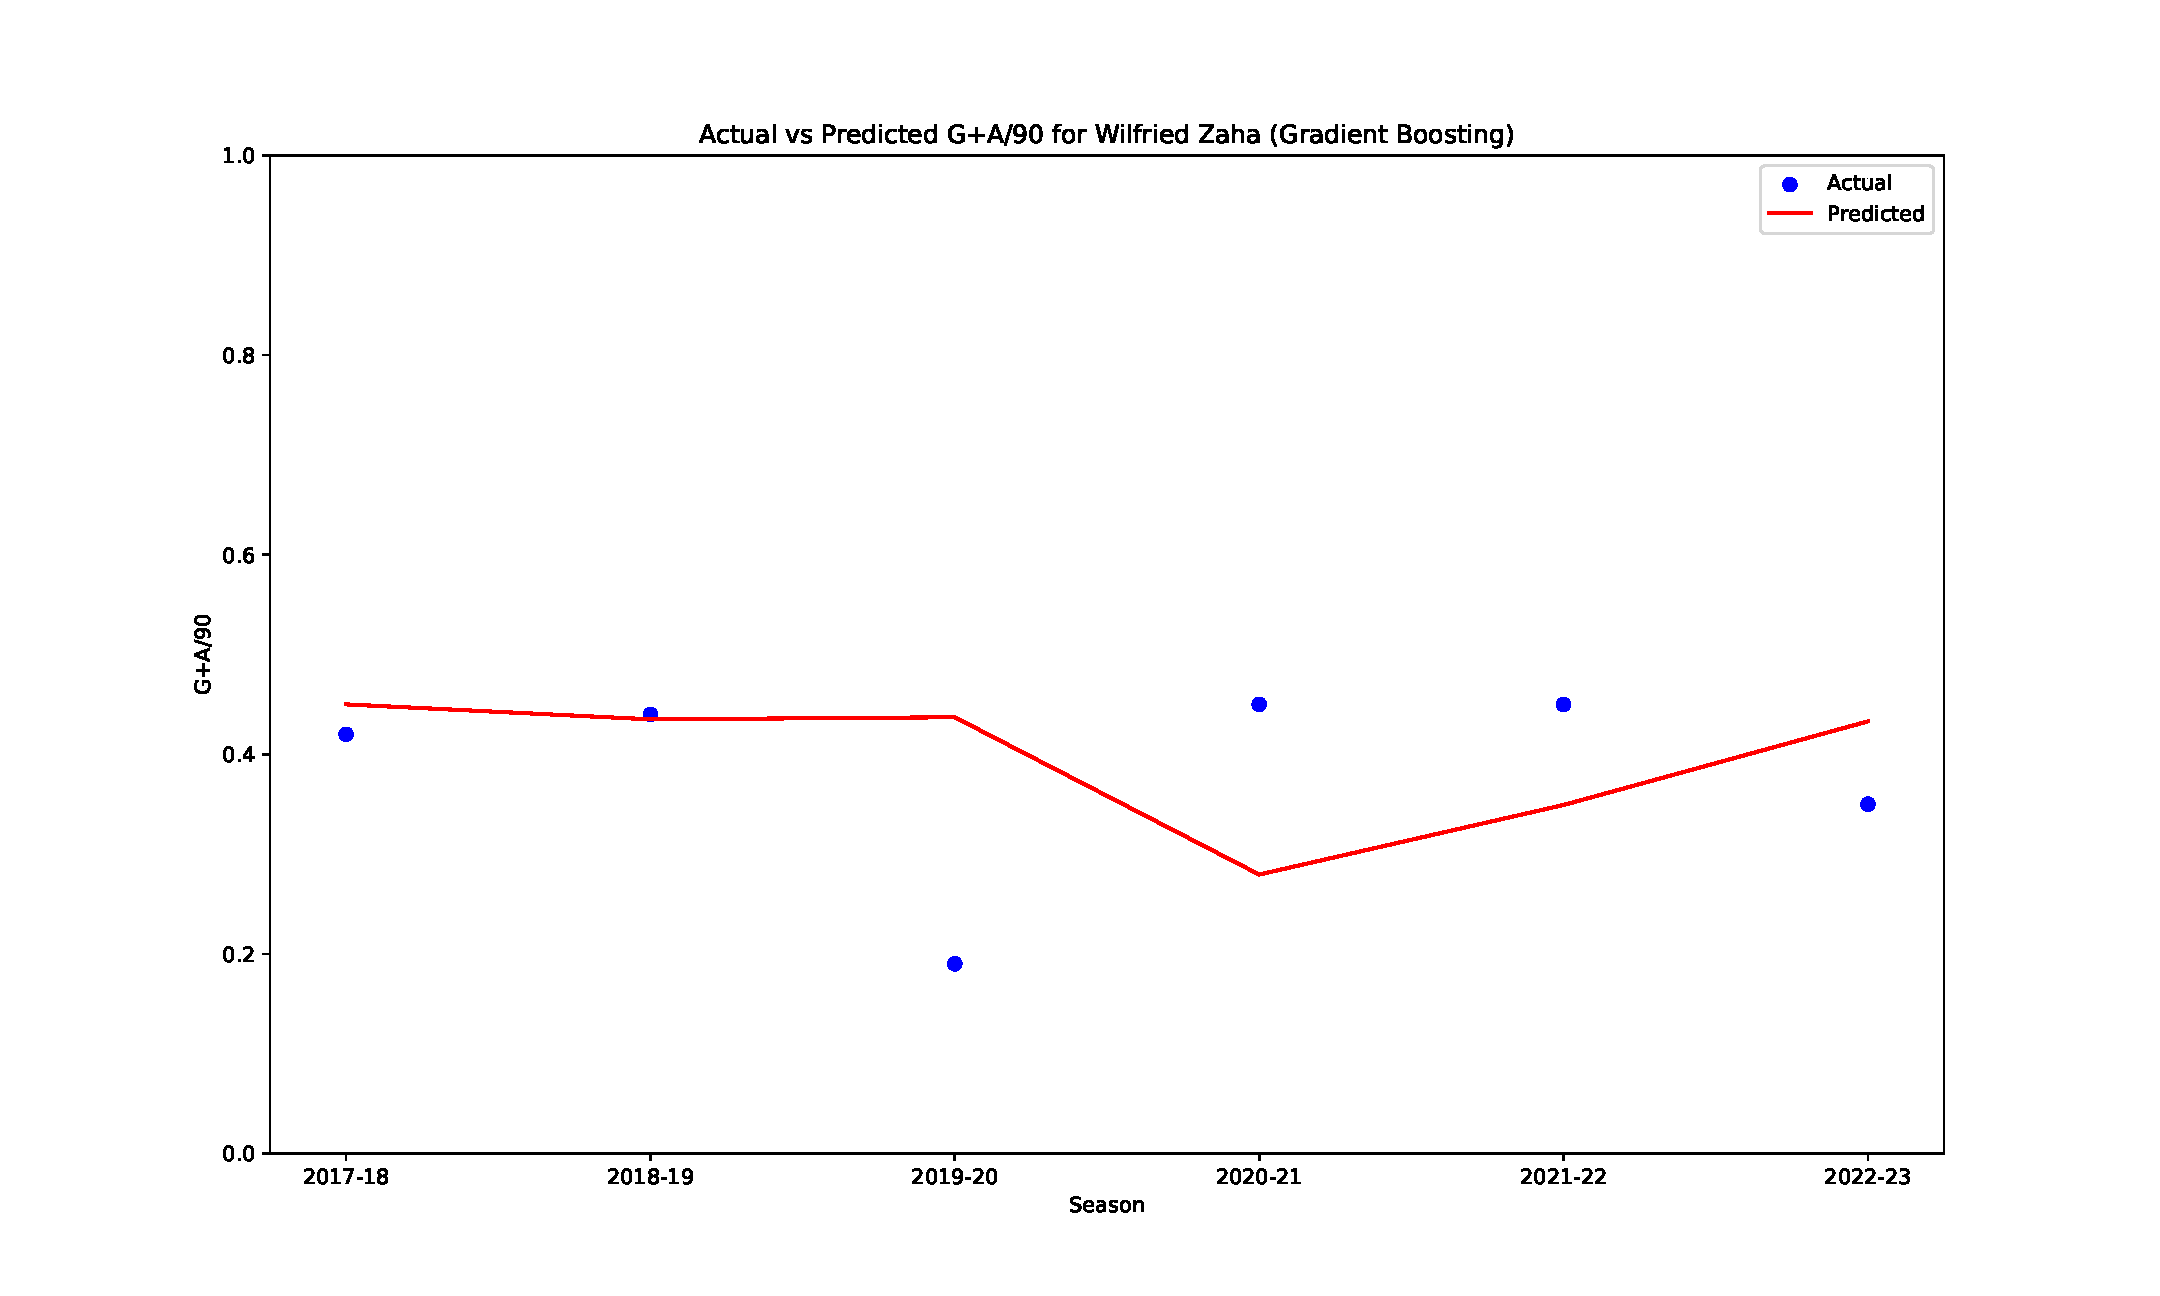
\includegraphics[width=1\textwidth]{GradBoost_Zaha.pdf}
  \caption{Wilfried Zaha Predictions vs Actual (Gradient Boost)}
  \label{fig:Zaha_graph}
  \end{figure}


%zaha acc vs pred
\begin{table}[H]
  \centering
  \begin{tabular}{|l|c|c|c|c|}
  \hline
  \textbf{Season} & \textbf{Actual G+A/90} & \textbf{Predicted G+A/90} & \textbf{Discrepancy} \\
  \hline
  2017-18 & 0.420 & 0.450 & 0.030 \\
  2018-19 & 0.440 & 0.435 & 0.005 \\
  2019-20 & 0.190 & 0.437 & 0.247 \\
  2020-21 & 0.450 & 0.279 & 0.171 \\
  2021-22 & 0.450 & 0.349 & 0.101 \\
  2022-23 & 0.350 & 0.433 & 0.083 \\
  \hline
  \end{tabular}
  \caption{Prediction Results for Wilfried Zaha}
  \label{tab:zaha_prediction_results}
  \end{table}
  

% Henderson fig
\begin{figure}[H]
  \centering
  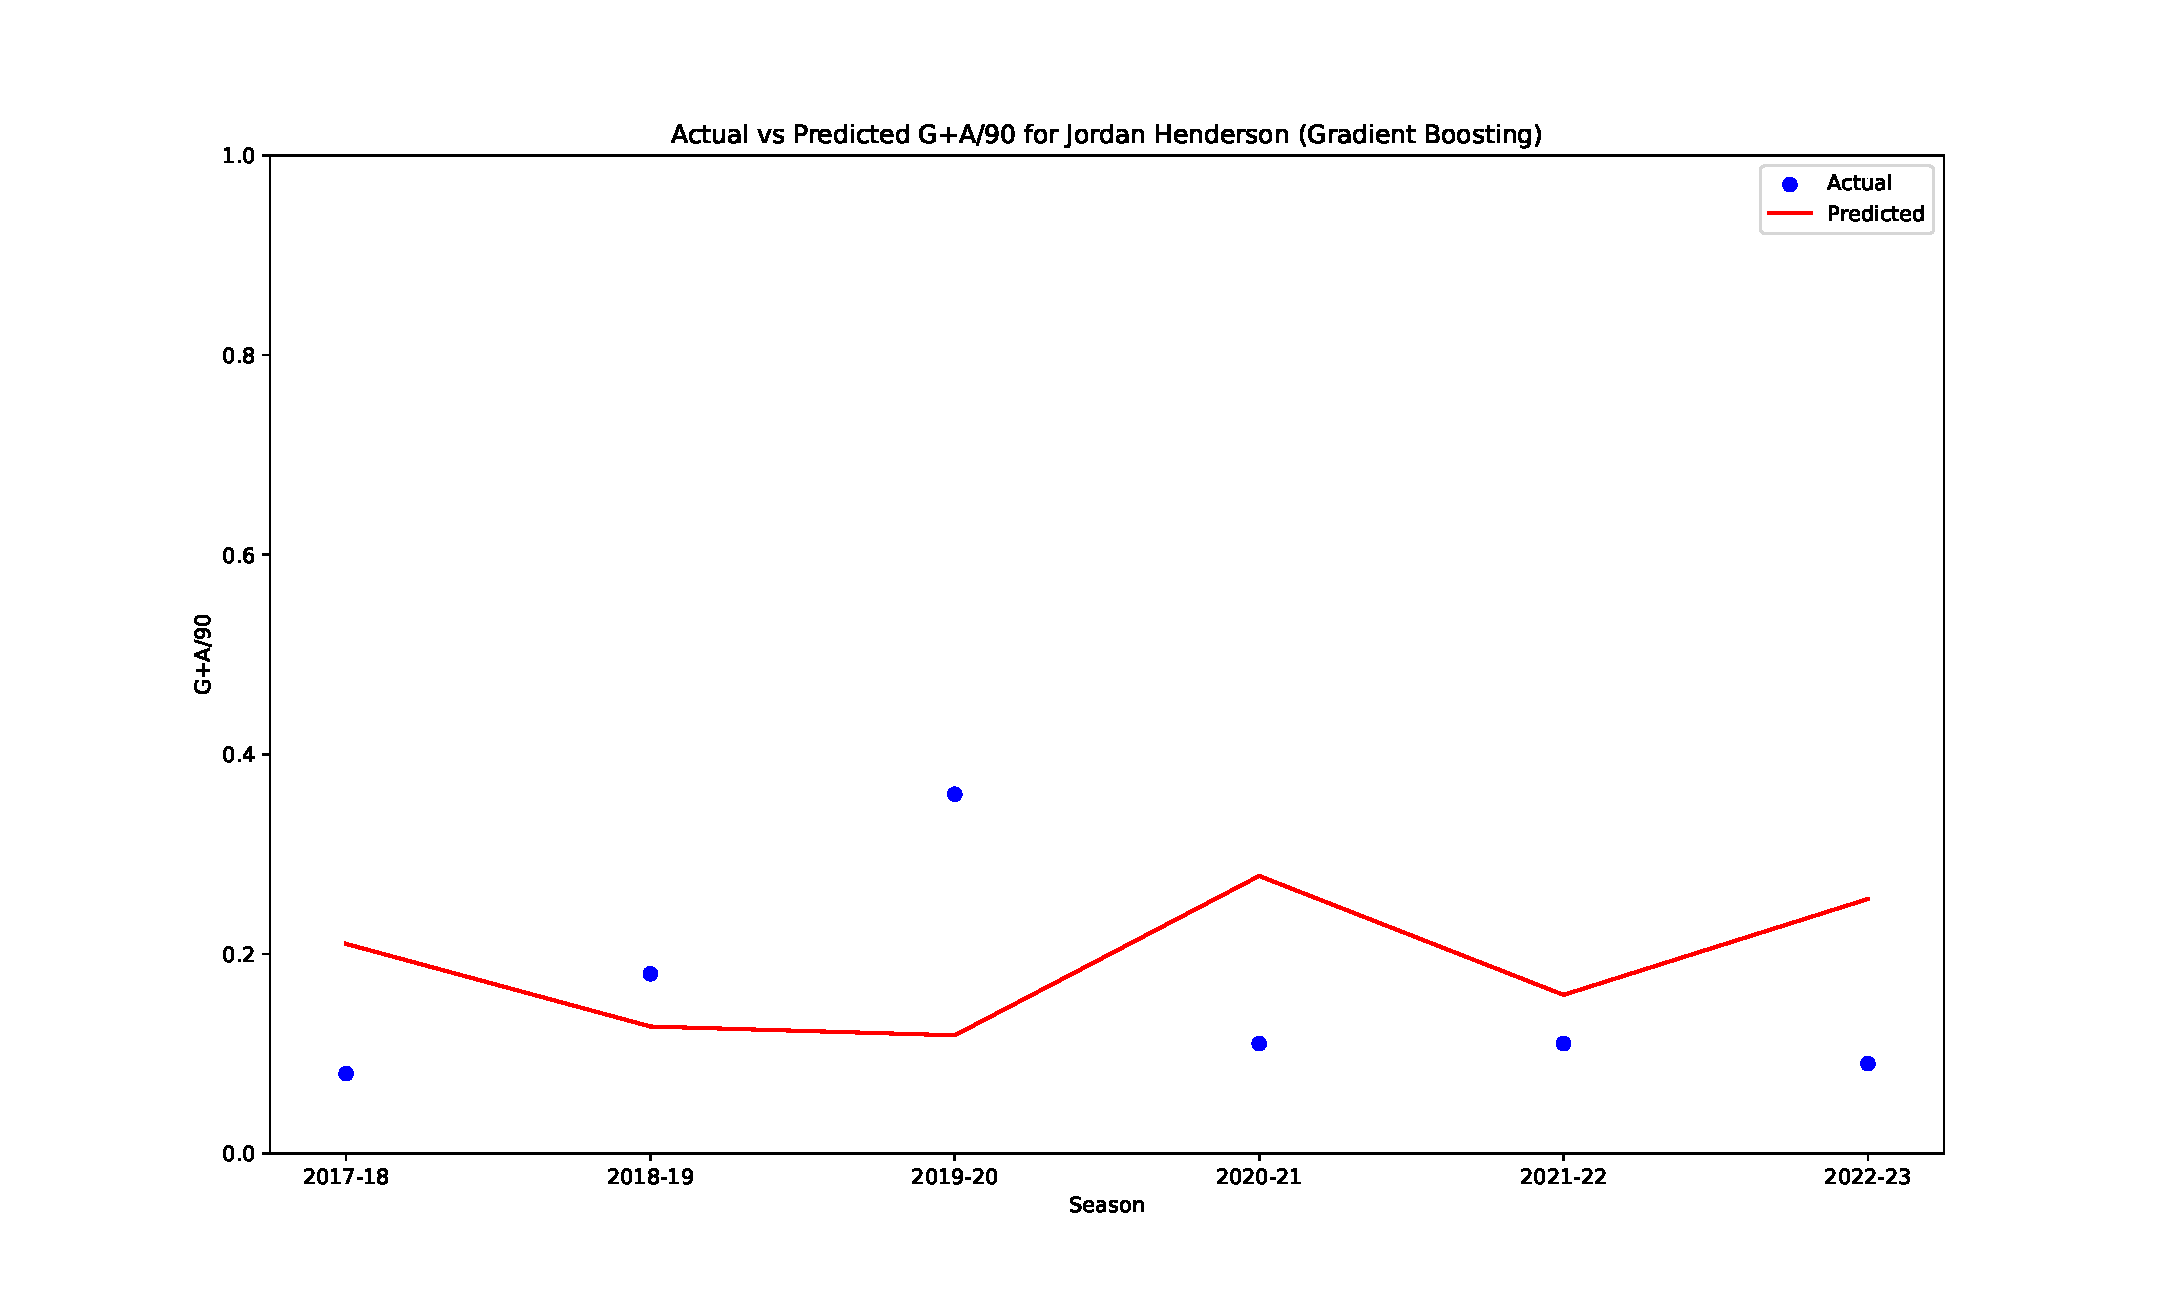
\includegraphics[width=1\textwidth]{GradBoost_Henderson.pdf}
  \caption{Jordan Henderson Predictions vs Actual (Gradient Boost)}
  \label{fig:Henderson_graph}
  \end{figure}

% Henderson Table

\begin{table}[H]
  \centering
  \begin{tabular}{|l|c|c|c|c|}
  \hline
  \textbf{Season} & \textbf{Actual G+A/90} & \textbf{Predicted G+A/90} & \textbf{Discrepancy} \\
  \hline
  2017-18 & 0.080 & 0.210 & 0.130 \\
  2018-19 & 0.180 & 0.127 & 0.053 \\
  2019-20 & 0.360 & 0.118 & 0.242 \\
  2020-21 & 0.110 & 0.278 & 0.168 \\
  2021-22 & 0.110 & 0.159 & 0.049 \\
  2022-23 & 0.090 & 0.255 & 0.165 \\
  \hline
  \end{tabular}
  \caption{Prediction Results for Jordan Henderson}
  \label{tab:henderson_prediction_results}
\end{table}

% kane figure

\begin{figure}[H]
  \centering
  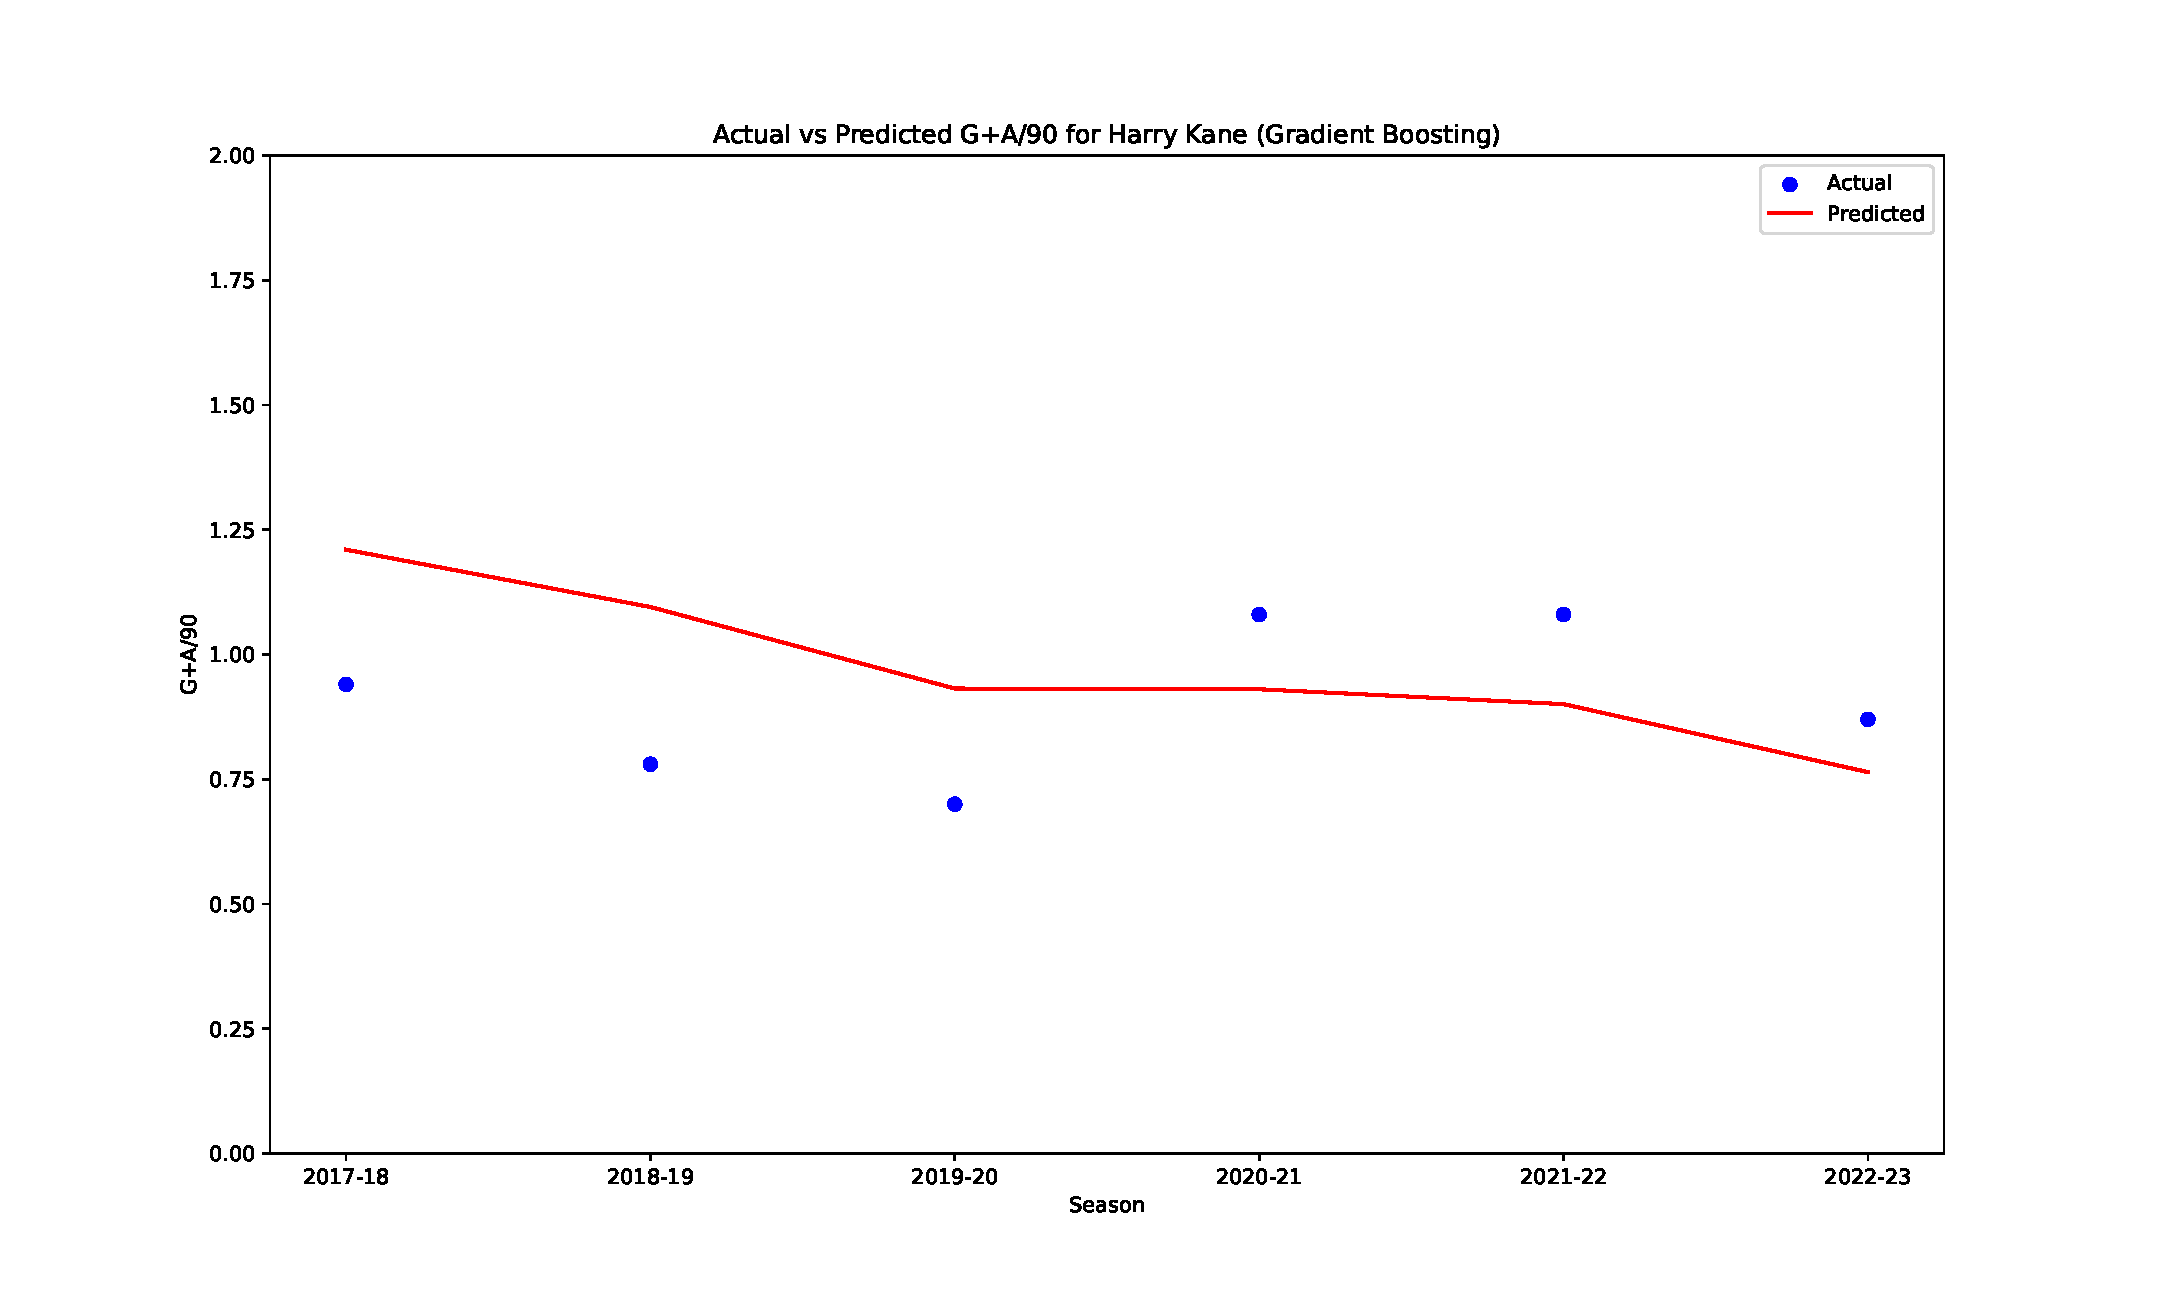
\includegraphics[width=1\textwidth]{GradBoost_Kane.pdf}
  \caption{Harry Kane Predictions vs Actual (Gradient Boost)}
  \label{fig:Kane_graph}
  \end{figure}

% Kane Table

  \begin{table}[H]
    \centering
    \begin{tabular}{|c|c|c|c|}
    \hline
    \textbf{Season} & \textbf{Actual G+A/90} & \textbf{Predicted G+A/90} & \textbf{Discrepancy} \\
    \hline
    2017-18 & 0.940 & 1.210 & 0.270 \\
    2018-19 & 0.780 & 1.095 & 0.315 \\
    2019-20 & 0.700 & 0.932 & 0.232 \\
    2020-21 & 1.080 & 0.930 & 0.150 \\
    2021-22 & 1.080 & 0.900 & 0.180 \\
    2022-23 & 0.870 & 0.764 & 0.106 \\
    \hline
    \end{tabular}
    \caption{Prediction Results for Harry Kane}
    \label{tab:kane_prediction_results}
  \end{table}
  
% Lallana figure

\begin{figure}[H]
  \centering
  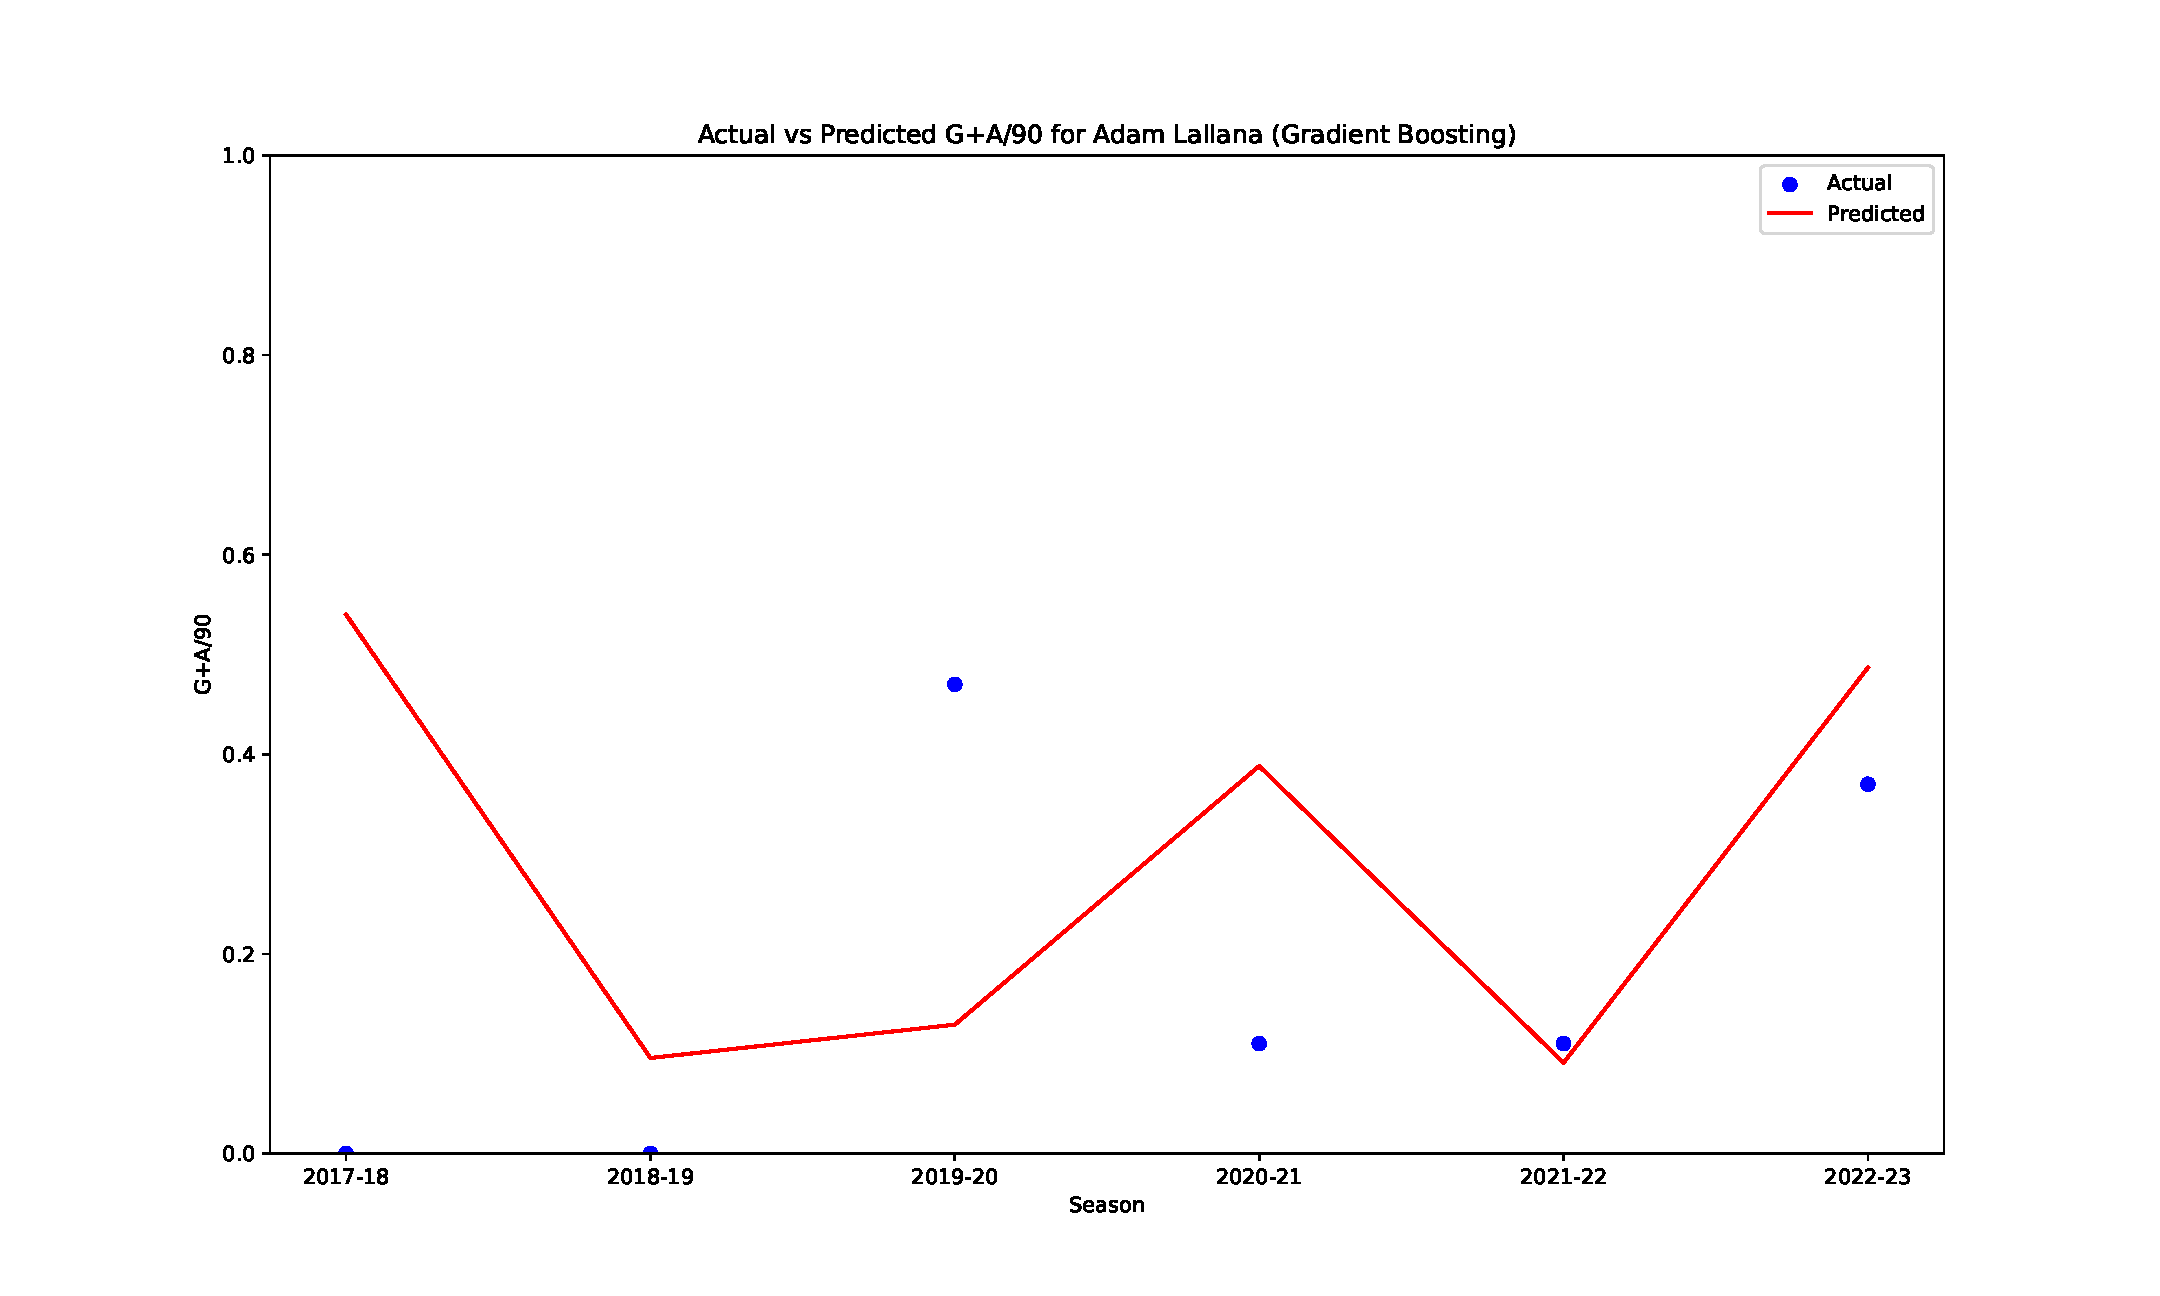
\includegraphics[width=1\textwidth]{GradBoost_Lallana.pdf}
  \caption{Adam Lallana Predictions vs Actual (Gradient Boost)}
  \label{fig:Lallana_graph}
  \end{figure}

% Lallana table

\begin{table}[H]
  \centering
  \begin{tabular}{|c|c|c|c|}
  \hline
  \textbf{Season} & \textbf{Actual G+A/90} & \textbf{Predicted G+A/90} & \textbf{Discrepancy} \\
  \hline
  2017-18 & 0.000 & 0.540 & 0.540 \\
  2018-19 & 0.000 & 0.096 & 0.096 \\
  2019-20 & 0.470 & 0.129 & 0.341 \\
  2020-21 & 0.110 & 0.388 & 0.278 \\
  2021-22 & 0.110 & 0.091 & 0.019 \\
  2022-23 & 0.370 & 0.487 & 0.117 \\
  \hline
  \end{tabular}
  \caption{Prediction Results for Adam Lallana}
  \label{tab:lallana_prediction_results}
\end{table}

% Chamberlain figure

\begin{figure}[H]
  \centering
  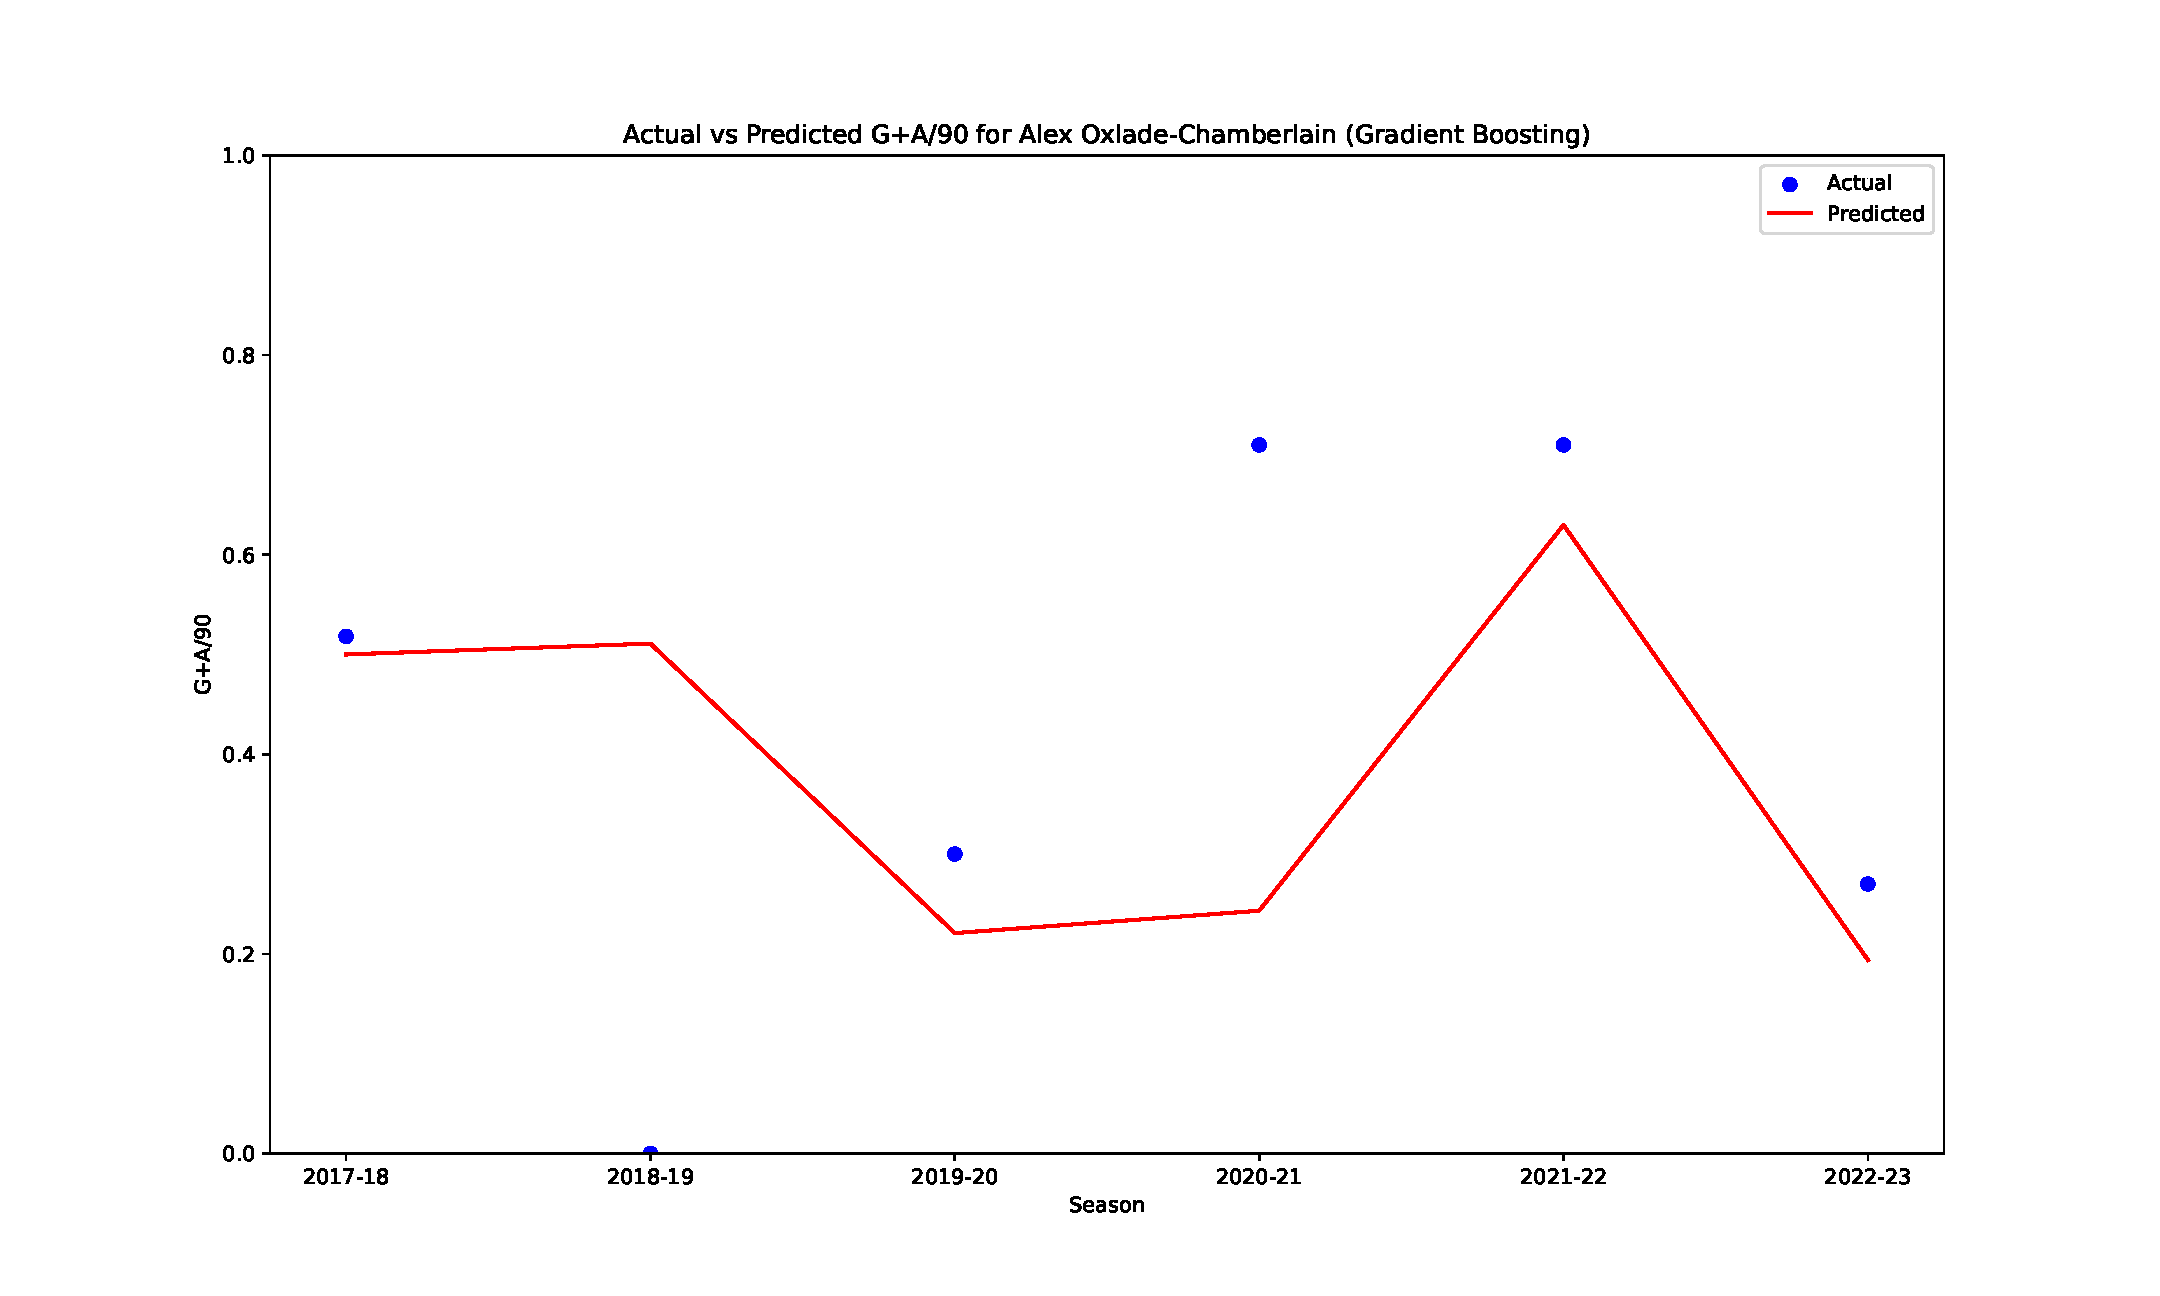
\includegraphics[width=1\textwidth]{GradBoost_Chamberlain.pdf}
  \caption{Alex Oxlade-Chamberlain Predictions vs Actual (Gradient Boost)}
  \label{fig:Chamberlain_graph}
  \end{figure}

% chamberlain table

\begin{table}[H]
  \centering
  \begin{tabular}{|c|c|c|c|}
  \hline
  \textbf{Season} & \textbf{Actual G+A/90} & \textbf{Predicted G+A/90} & \textbf{Discrepancy} \\
  \hline
  2017-18 & 0.518 & 0.500 & 0.018 \\
  2018-19 & 0.000 & 0.511 & 0.511 \\
  2019-20 & 0.300 & 0.221 & 0.079 \\
  2020-21 & 0.710 & 0.243 & 0.467 \\
  2021-22 & 0.710 & 0.630 & 0.080 \\
  2022-23 & 0.270 & 0.194 & 0.076 \\
  \hline
  \end{tabular}
  \caption{Prediction Results for Alex Oxlade-Chamberlain}
  \label{tab:oxlade_chamberlain_prediction_results}
\end{table}

% Sterling figure

\begin{figure}[H]
  \centering
  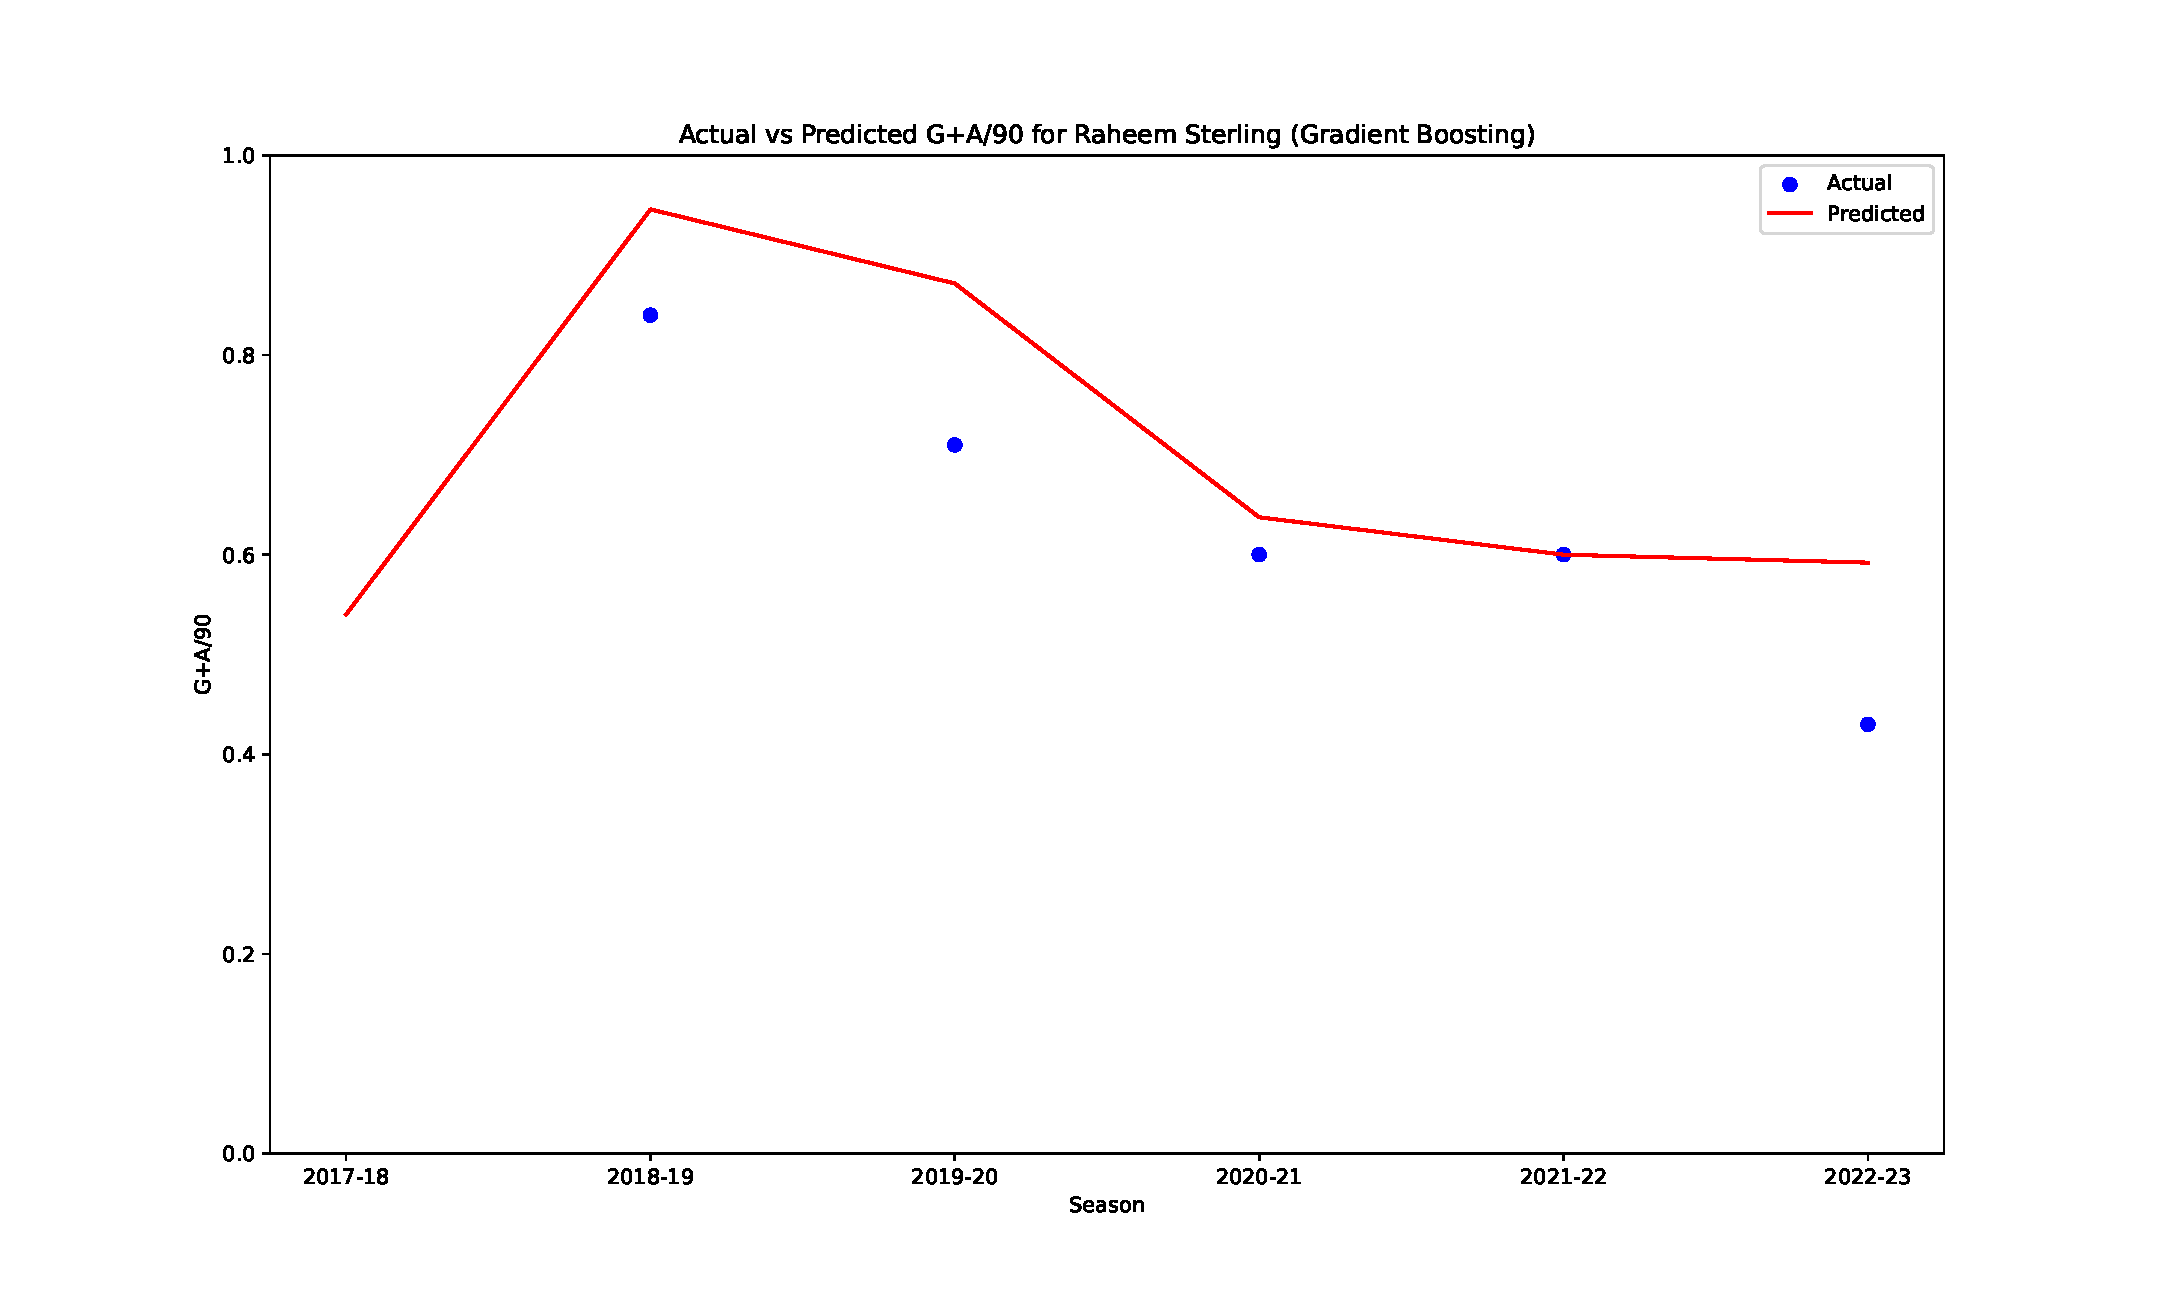
\includegraphics[width=1\textwidth]{GradBoost_Sterling.pdf}
  \caption{Raheem Sterling Predictions vs Actual (Gradient Boost)}
  \label{fig:Sterling_graph}
  \end{figure}

% Sterling Table

  \begin{table}[H]
    \centering
    \begin{tabular}{|c|c|c|c|}
    \hline
    \textbf{Season} & \textbf{Actual G+A/90} & \textbf{Predicted G+A/90} & \textbf{Discrepancy} \\
    \hline
    2017-18 & 1.010 & 0.540 & 0.470 \\
    2018-19 & 0.840 & 0.946 & 0.106 \\
    2019-20 & 0.710 & 0.872 & 0.138 \\
    2020-21 & 0.600 & 0.637 & 0.037 \\
    2021-22 & 0.600 & 0.600 & 0.000 \\
    2022-23 & 0.430 & 0.592 & 0.162 \\
    \hline
    \end{tabular}
    \caption{Prediction Results for Raheem Sterling}
    \label{tab:sterling_prediction_results}
  \end{table}

  % Welbeck Graph
  \begin{figure}[H]
    \centering
    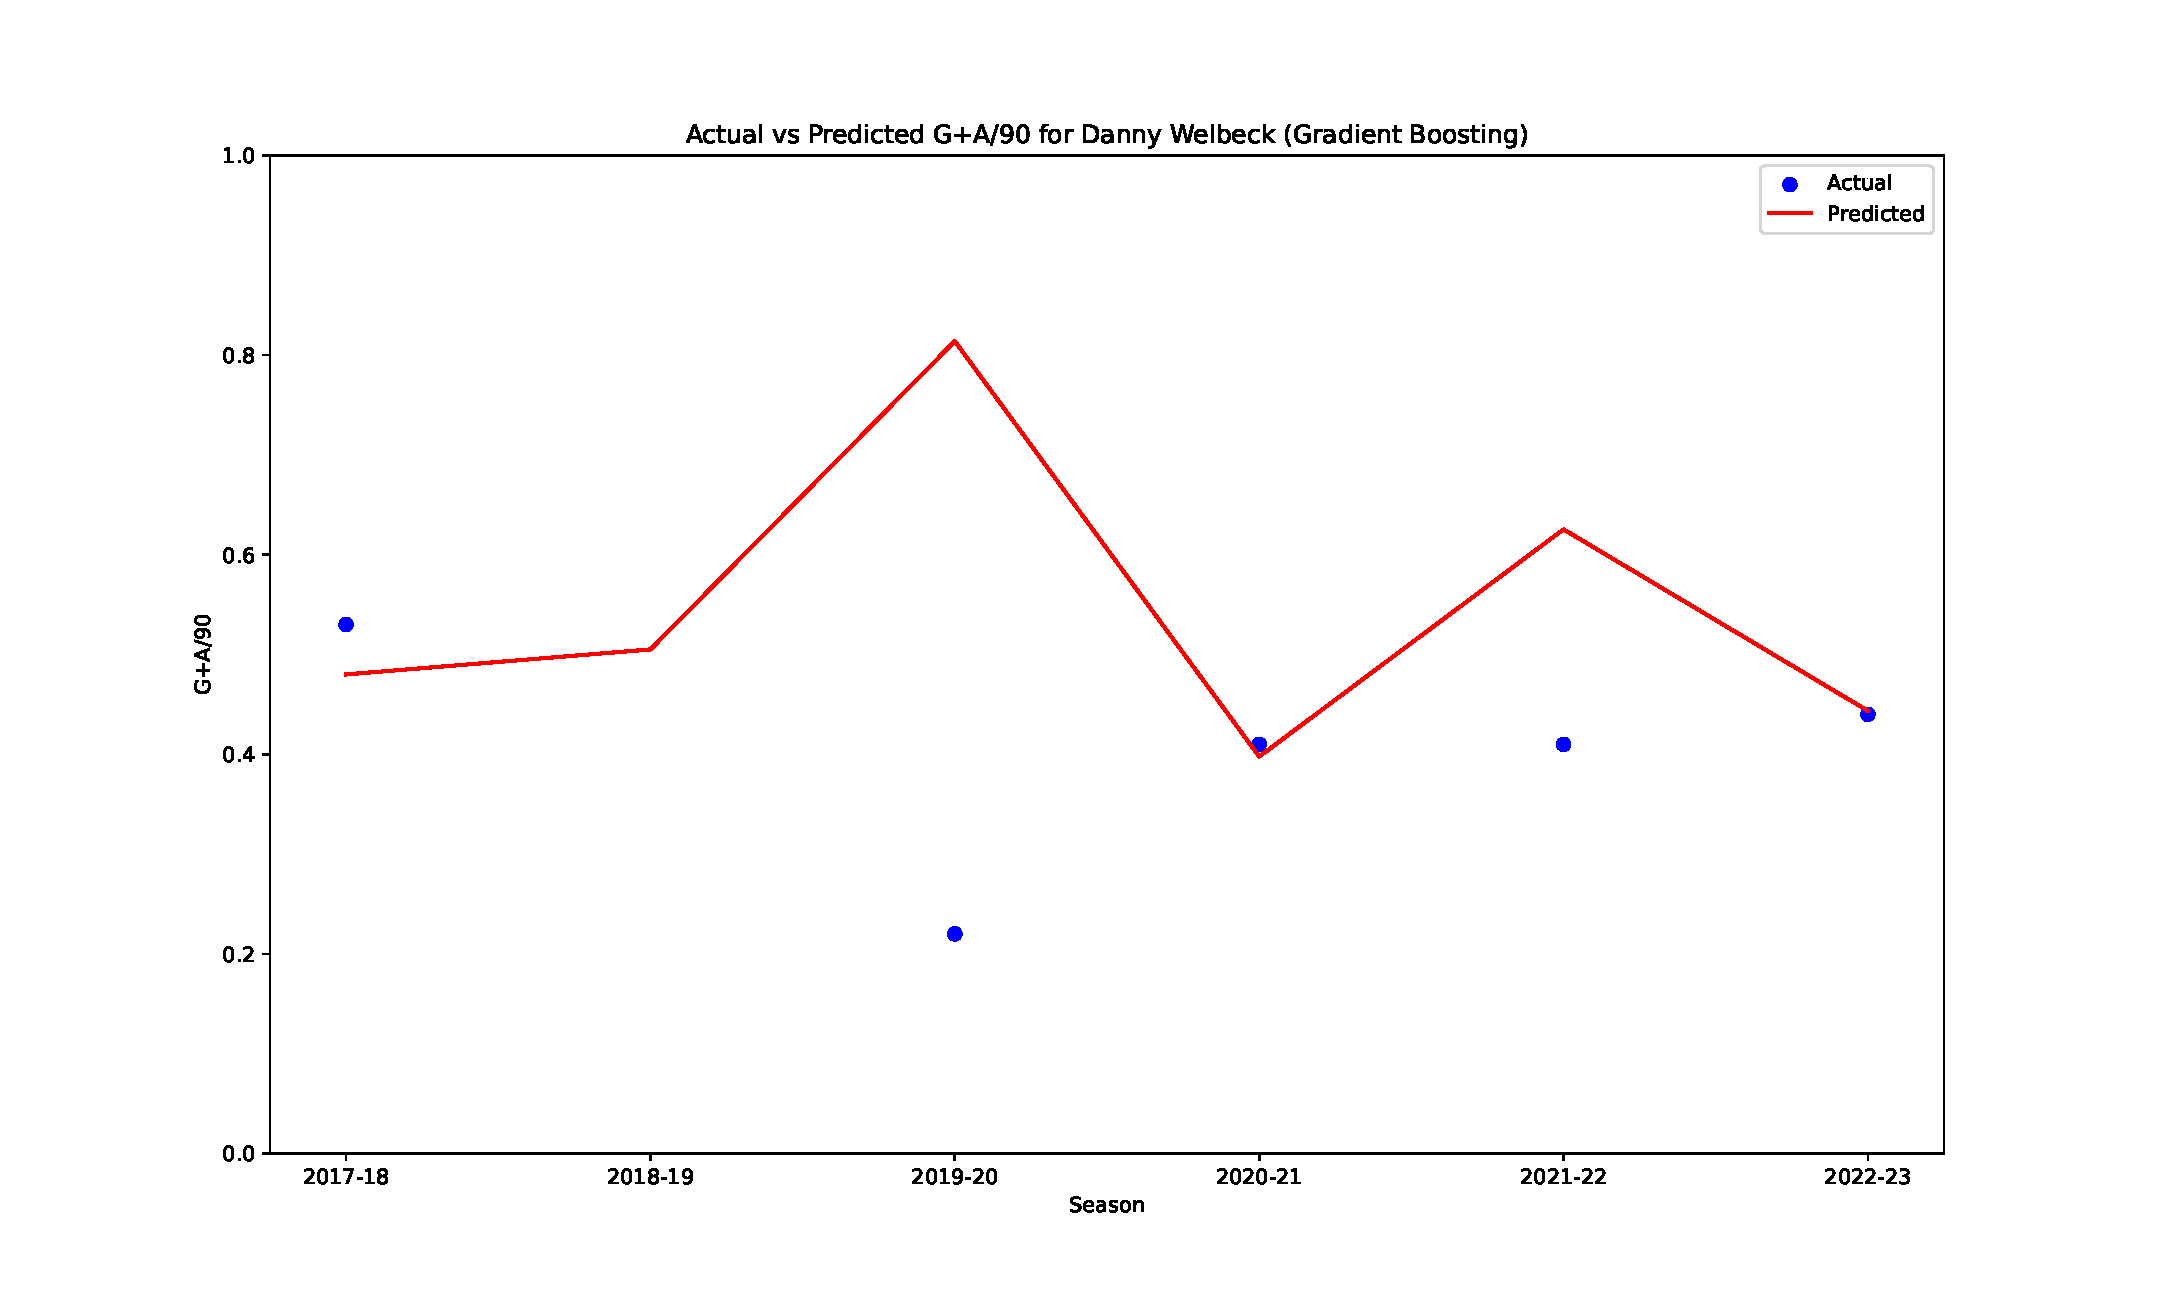
\includegraphics[width=1\textwidth]{GradBoost_Welbeck.pdf}
    \caption{Danny Welbeck Predictions vs Actual (Gradient Boost)}
    \label{fig:Welbeck_graph}
    \end{figure}

  % Welbeck table


    \begin{table}[H]
      \centering
      \begin{tabular}{|c|c|c|c|}
      \hline
      \textbf{Season} & \textbf{Actual G+A/90} & \textbf{Predicted G+A/90} & \textbf{Discrepancy} \\
      \hline
      2017-18 & 0.530 & 0.480 & 0.050 \\
      2018-19 & 1.180 & 0.505 & 0.675 \\
      2019-20 & 0.220 & 0.814 & 0.594 \\
      2020-21 & 0.410 & 0.398 & 0.012 \\
      2021-22 & 0.410 & 0.625 & 0.215 \\
      2022-23 & 0.440 & 0.444 & 0.004 \\
      \hline
      \end{tabular}
      \caption{Prediction Results for Danny Welbeck}
      \label{tab:welbeck_prediction_results}
    \end{table}
    
  
% Ward Prowse figure
\begin{figure}[H]
  \centering
  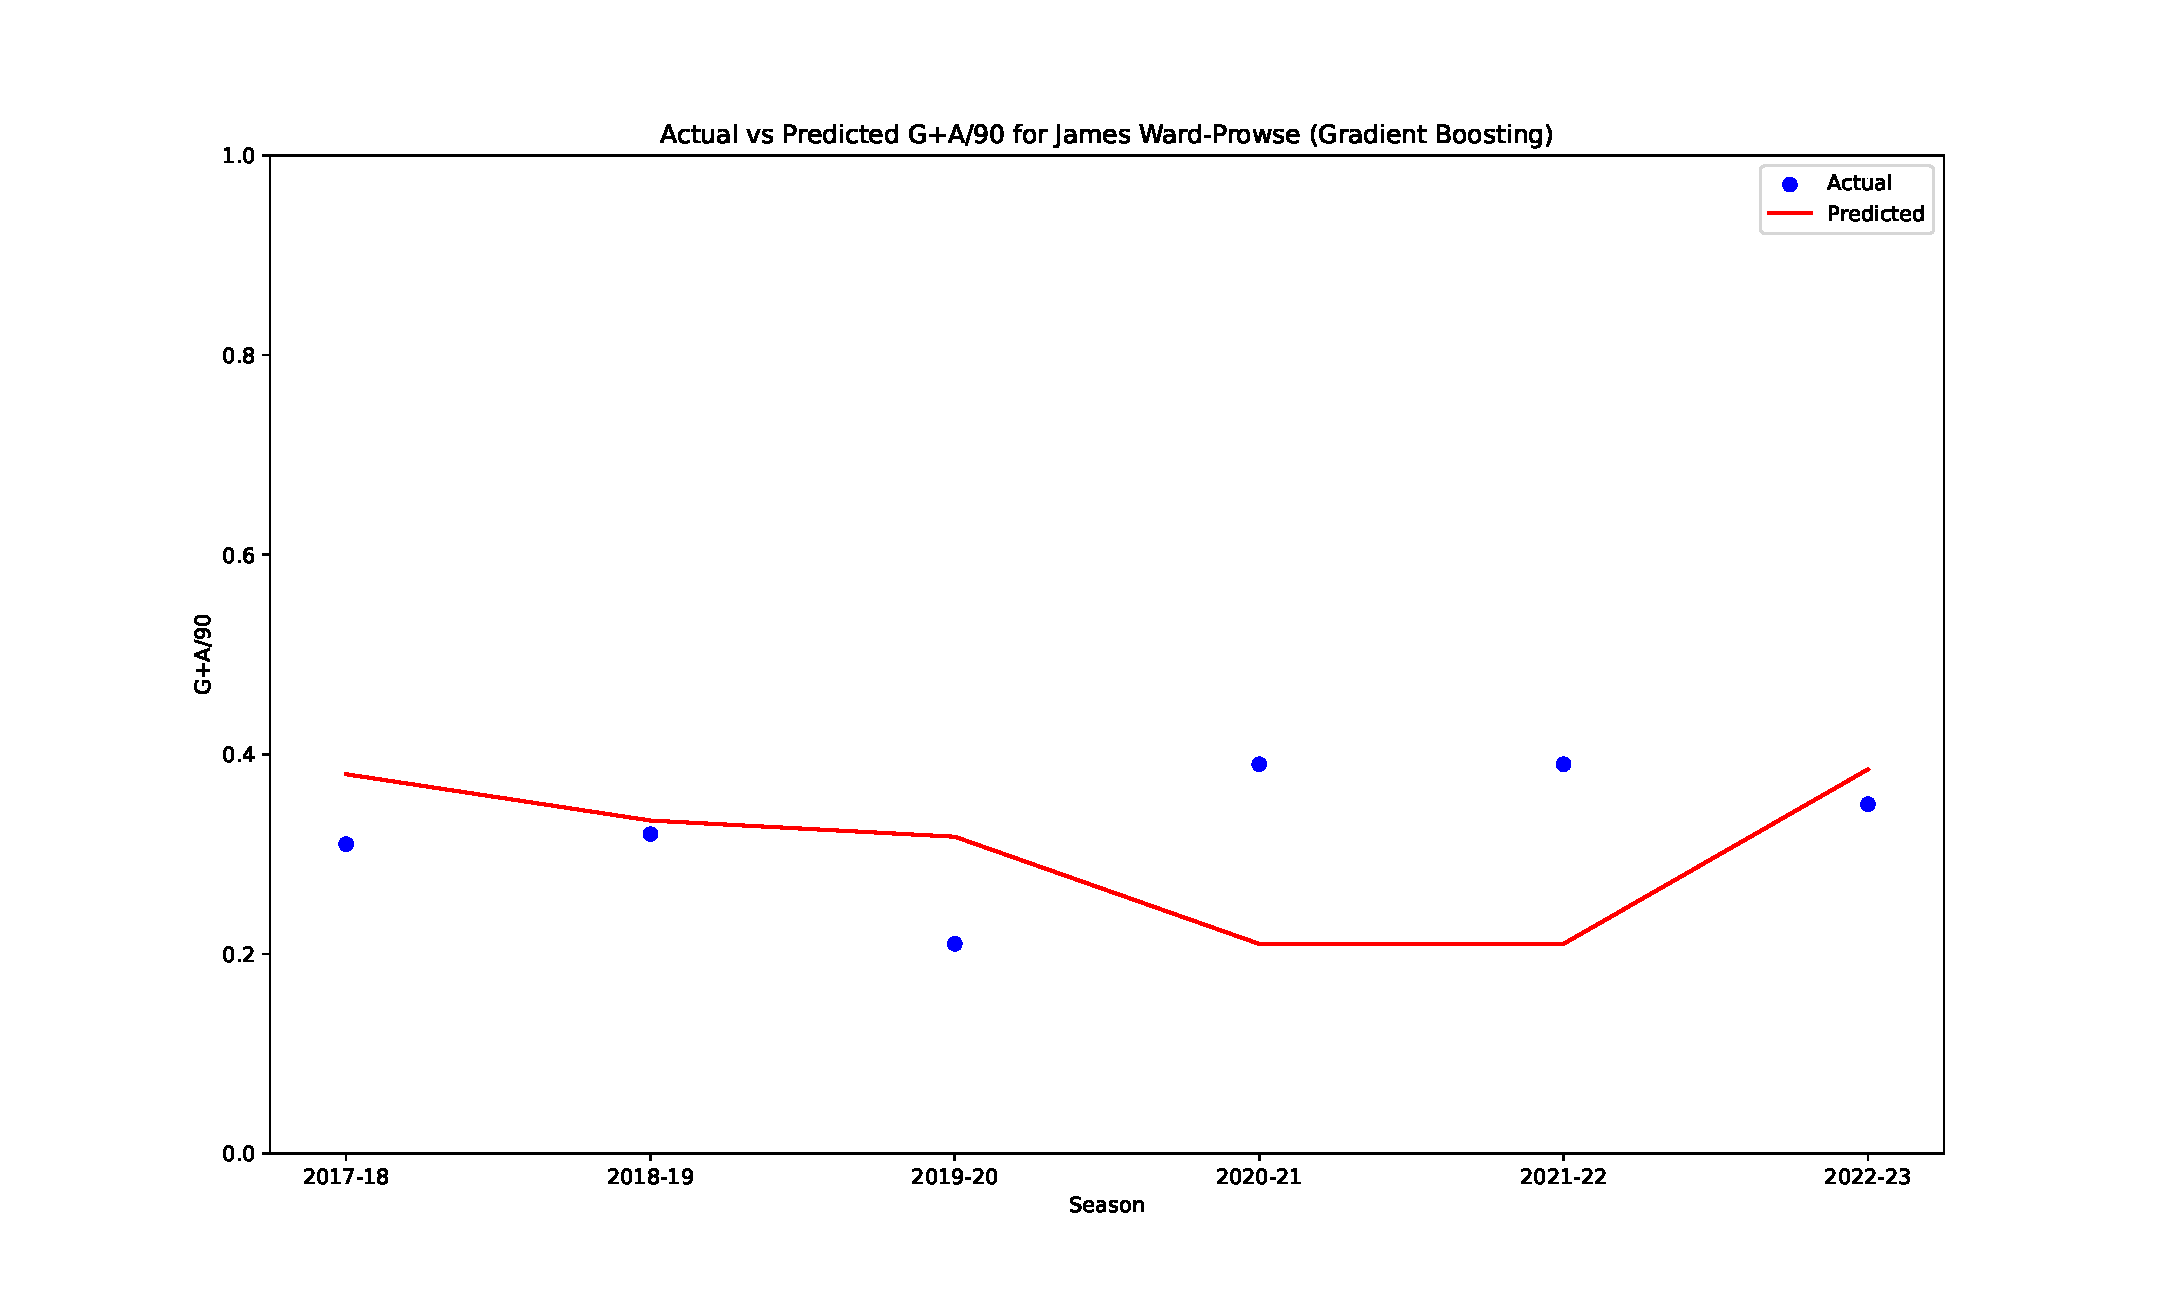
\includegraphics[width=1\textwidth]{GradBoost_Prowse.pdf}
  \caption{James Ward-Prowse Predictions vs Actual (Gradient Boost)}
  \label{fig:Prowse_graph}
  \end{figure}

% ward prowse table

\begin{table}[h]
  \centering
  \begin{tabular}{|c|c|c|c|}
  \hline
  \textbf{Season} & \textbf{Actual G+A/90} & \textbf{Predicted G+A/90} & \textbf{Discrepancy} \\
  \hline
  2017-18 & 0.310 & 0.380 & 0.070 \\
  2018-19 & 0.320 & 0.334 & 0.014 \\
  2019-20 & 0.210 & 0.317 & 0.107 \\
  2020-21 & 0.390 & 0.210 & 0.180 \\
  2021-22 & 0.390 & 0.210 & 0.180 \\
  2022-23 & 0.350 & 0.385 & 0.035 \\
  \hline
  \end{tabular}
  \caption{Prediction Results for James Ward-Prowse}
  \label{tab:wardprowse_prediction_results}
\end{table}

% walcott figure
\begin{figure}[H]
  \centering
  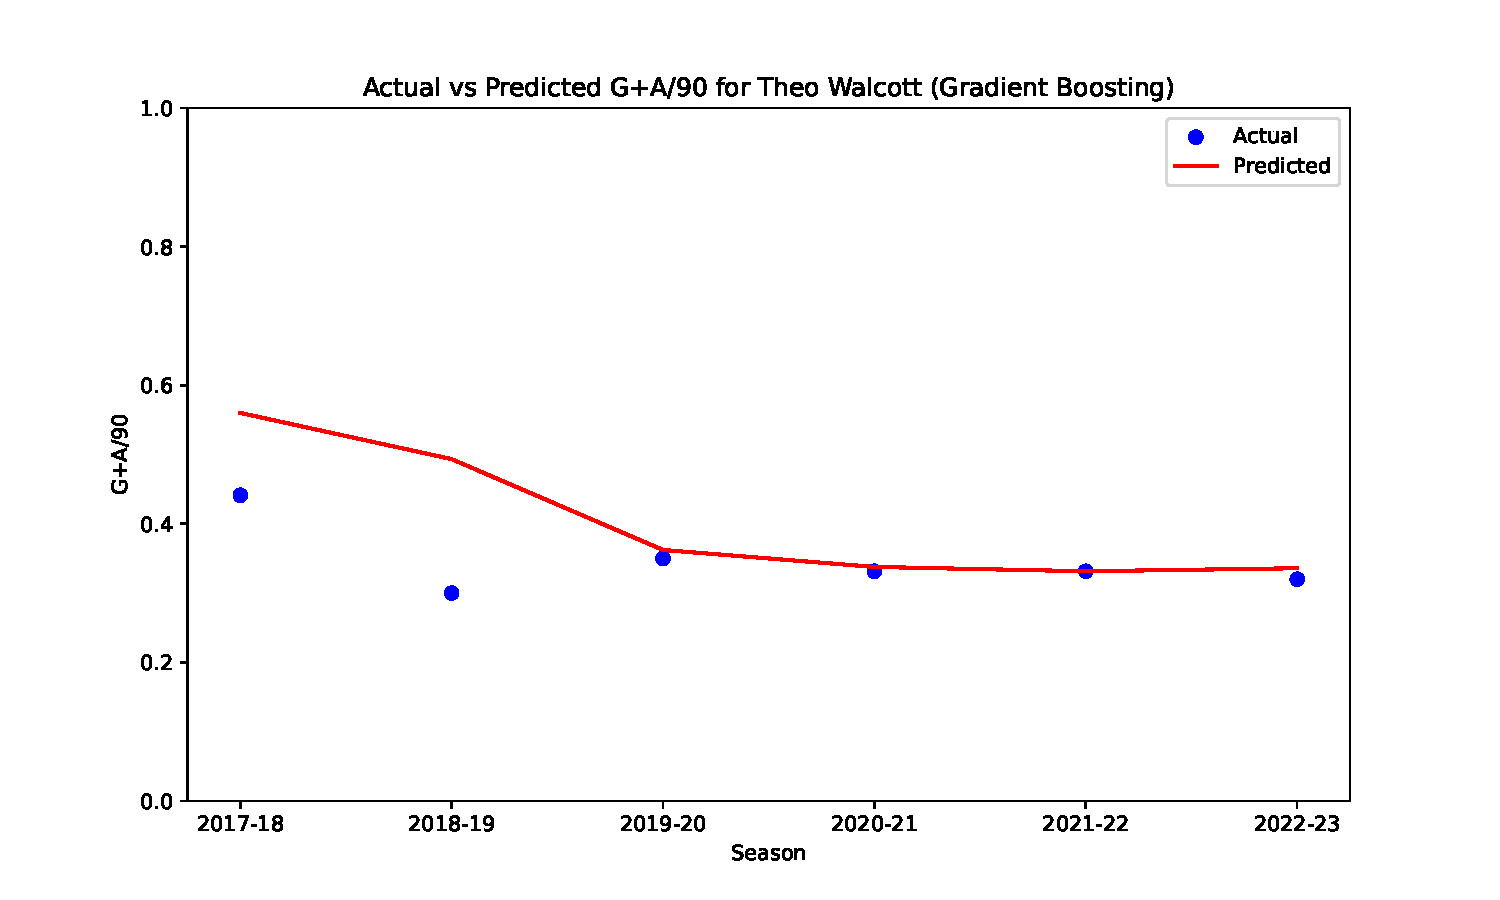
\includegraphics[width=1\textwidth]{GradBoost_Walcott.pdf}
  \caption{Theo Walcott Predictions vs Actual (Gradient Boost)}
  \label{fig:Walcott_graph}
  \end{figure}


% walcott table

\begin{table}[h]
  \centering
  \begin{tabular}{|c|c|c|c|}
  \hline
  \textbf{Season} & \textbf{Actual G+A/90} & \textbf{Predicted G+A/90} & \textbf{Discrepancy} \\
  \hline
  2017-18 & 0.441 & 0.560 & 0.119 \\
  2018-19 & 0.300 & 0.493 & 0.193 \\
  2019-20 & 0.350 & 0.362 & 0.012 \\
  2020-21 & 0.331 & 0.338 & 0.007 \\
  2021-22 & 0.331 & 0.331 & 0.000 \\
  2022-23 & 0.320 & 0.336 & 0.016 \\
  \hline
  \end{tabular}
  \caption{Prediction Results for Theo Walcott}
  \label{tab:walcott_prediction_results}
\end{table}


% overall performance of grad boost

\begin{table}[H]
  \centering
  \begin{tabular}{|l|c|c|c|}
  \hline
  \textbf{Player Name} & \textbf{MSE} & \textbf{MAE} & \textbf{Correlation} \\
  \hline
  Wilfried Zaha & 0.018 & 0.106 & -0.457 \\
  Jordan Henderson & 0.023 & 0.134 & -0.689 \\
  Harry Kane & 0.049 & 0.209 & -0.093 \\
  Adam Lallana & 0.085 & 0.232 & -0.060 \\
  Alex Oxlade-Chamberlain & 0.083 & 0.205 & 0.141 \\
  Raheem Sterling & 0.048 & 0.156 & 0.186 \\
  Danny Welbeck & 0.143 & 0.258 & -0.362 \\
  James Ward-Prowse & 0.014 & 0.098 & -0.495 \\
  Theo Walcott & 0.009 & 0.058 & 0.589 \\
  \hline
  \end{tabular}
  \caption{Gradient Boost Evaluation Metrics for Each Player}
  \label{tab:player_evaluation_metrics}
\end{table}






\section{Discussion}
\label{sec:disc}

% What are the main contributions again?

% What are the limitations of this study?

% What are worth pursuing further in the future?

The evalutation 
metrics we used to compare the performance of our models were Mean Squared Error
(MSE), Mean Absolute Error (MAE) and Correlation (Corr). These values for each 
model were calculated by taking the averages of these values for each player
thus providing an insight of how the model performed in its predictions of all 
9 players in this investigation. MSE and MAE give a sense of the magnitude
of errors with lower values indicating better performance, while correlation
provides insight into the linear relationship between predicted and actual values
with values closer to 1 or -1 indicating a stronger linear relationship.
For our study, higher signifcance in evaluating model performance is placed on
the MSE and MAE values as they give a clearer indication on prediction accuracy 
against actual player performance. Correlation will hold less weight in 
our best model selection due to the fact that we do not necessarily expect player 
performance to be especially linear. The main focus is getting as near to the 
correct values as possible.

As we can see from Table \ref{tab:model_performance} which compared all 6
potential models for carrying out our investigation, the prediction model with
the lowest average MSE (MSE = 0.041) and MAE (MAE = 0.150) was Gradient Boosting,
thus becoming the model used to carry out our player predictions.

From Table \ref{tab:player_evaluation_metrics} we can see the MSE, MAE and Corr 
for each player in which the Gradient Boosting prediciton model was applied.
We see that the player which our model was able to most accurately predict was 
Theo Walcott as this set of results had the lowest MSE (MSE = 0.009) and MAE
(MAE = 0.058) values. The player that the model did the worst with prediciting
was Danny Welbeck as this set of results had the highest MSE (MSE =0.143) and 
and the highest MAE (MAE = 0.258).

From this we can see that our model expressed good proficiency is predicting 
the goal contributions of each player based on historical data as shown by the 
relatively low average MSE and MAE values, showing that on average the  model's
predictions are close to the actual values in terms of magnitude. This  is
indicative of the model's ability to capture the general trends and patterns
present in the data. 
In relation to our central research question- "How does historical player
performance data, including key performance metrics, influence the prediction of
player's goal contributions per 90 minutes in future Premier League soccer matches,
and how can this information be leveraged for strategic decision-making?" - upon
the results of research, we can state that previous historical performance data 
such as goal contributions per 90 minutes as well as variables such as age, 
position and minutes played provides enough substantial input to make proficiently 
accurate predictions on player's future goal contributions per 90 minutes and 
consequently can be used to guide decision making regarding specific player 
performance statisitcs.
The results of this study falls in line with other literature in the field of 
predicitve modelling within sport such as the previously mentioned work of 
\citet{geurkink2021machine} who also used Gradient Boosting in their research,
resulting in a model accuracy of approximately 90\%. This shows that although 
performance model should not be soley relied upon, they  are able to provide
proficiently accurate predicitions for the majority of circumstances and thus can
definitely be used to inform and guide decision making within sporting contexts.

However, there are some limitations to be addressed with this type of research.
When it comes to player performance, due to the nature of sport there are always
going to be intangible variables which we are not able to account for in any type 
of quantitative research which can affect indivdual performance. An example of
one of these intagible variables would be confidence. The level of confidence 
in a player's own abilities can not only vary from season to season but from game to 
game and can fluctuate due to numerous factors. Variables such as confidence are 
extremely subjective and can be influenced by recent successes or failures,
team dynamics, and external pressures. Another such variable would be
motivation. An indivdual's drive to succeed, personal goals, and external
motivators can influence a player's effort and commitment, impacting their
overall performance. One again motivation can change from game to game and season 
by season. Other relevant intagible factors that further explain the limitations 
of our research include: focus and concentration, team chemistry, work ethic and 
team culture. These variables can all change on a season by season basis and due 
the fact they cannot be measured can help explain why our model at times made 
less accurate predictions on player performance.
The exisetence of intagible variables highlights the complexity and multifaceted
nature of player performance. These factors may interact in intricate ways,
which adds a layer of challenge to predicting performance based solely on historical
data and statistical models.

Another limitation with our research includes the influence of off-field variables.
Our research focused soley on on-field performance metrics that can be observed
in game. However, outside factors can have a significant
impact on performance and are typically harder to measure and evaluate.
An example of one of these off-field variables is injuries. 
Player injuries, both current and historical, can heavily influence performance.
The type, severity, and recovery time of injuries may have long-term effects on
a player's capabilities. Another vital off-field variable related to player
performance is recovery and rehabilitation. The effectiveness of a player's
recovery and rehabilitation processes can impact their return to optimal
performance levels. Factors such as access to quality medical care and adherence
to rehabilitation programs are crucial. Recovery and rehabilitation also
encapsulates aspects such as:

\begin{itemize}
  \item Nutrition and Diet: The quality of a player's nutrition and dietary habits can
  affect physical fitness, energy levels, and overall health, influencing
  performance on the field.
  \item Rest and Sleep: Adequate rest and quality sleep are essential for recovery and
  maintaining peak physical and mental performance. Sleep deprivation or irregular
  sleep patterns can negatively impact a player's abilities.
  \item Lifestyle Choices: Off-field lifestyle choices, including habits related to
  alcohol consumption, smoking, and recreational activities, can influence a
  player's overall well-being and, consequently, their performance.
\end{itemize}

Other relevant off-field variables include external stressors, media and public
pressure and contractual and transfer issues. Considering these off-field
variables is essential for a comprehensive understanding of player performance
and recognizing them helps us further understand the reasoning for our model
making less accurate predictions at times.

\subsection{Future Recommendations}

While this paper has provided valuable insights into the predictive modeling of
player performance in Premier League soccer matches using historical data, there
are several avenues for future research that can enhance the
comprehensiveness and applicability of such predictive models.

Firstly, future research could explore the inclusion of additional features to
improve the model's accuracy. Beyond the current set of performance metrics,
considering contextual factors such as match importance, team dynamics, and
opponent strength may provide a more nuanced understanding of player contributions.
Additionally, exploring advanced player tracking data, when available, could
offer richer insights into player movements and positioning during matches.

Feature expansion could extend beyond the quantitative metrics to include
intangible variables that significantly influence player performance. Variables
such as confidence, motivation, and psychological factors play a crucial role in
an athlete's on-field performance. Incorporating these intangible aspects into
the predictive model may unravel new dimensions of understanding, capturing the
intricacies of a player's mental state and its impact on their contributions.
Intangible aspects are challenging to quantify and measure directly. However,
while they may not be as easily captured as numerical statistics, there are
indirect methods and proxies that researchers can employ to incorporate some
aspects of these intangibles into predictive models.
Some suggestions include:

\begin{itemize}
  \item Survey Data: Conducting surveys or interviews with players, coaches, or
  other stakeholders can provide subjective insights into intangible factors.
  Questions related to confidence, motivation, and mental state can contribute
  qualitative data.
  \item Sentiment Analysis: Analyzing media reports, interviews, or social media
  content related to players can provide sentiment indicators. Positive or
  negative sentiments expressed in these sources may offer clues about a player's
  mental state.
  \item Performance in High-Pressure Situations: Assessing a player's historical
  performance in high-pressure or critical matches can indirectly reflect their
  mental resilience and composure during crucial moments.
  \item Leadership Roles: Examining a player's history of leadership roles within
   the team, such as being a captain, may provide insights into their influence
   on team dynamics beyond statistical contributions.
   \item Team Dynamics: Exploring team dynamics and interpersonal relationships
   can indirectly shed light on intangible factors. For instance, analyzing team
   cohesion, communication patterns, or changes in squad dynamics over time can
   offer context.
\end{itemize}

Furthermore, the study could benefit from a deeper investigation into off-field
variables. Injuries, for instance, are known to substantially affect a player's
performance, yet the current model does not explicitly account for such occurrences.
Future research could delve into injury data and incorporate it into the model
to better predict performance fluctuations resulting from players returning from
injuries or being sidelined.

To enhance the generalizability of the model, expanding the dataset to include
players from various leagues and regions could provide a more comprehensive
understanding of the factors influencing player performance. This cross-league
analysis could uncover patterns and trends that extend beyond the unique dynamics
of the Premier League.

Additionally, the temporal scope of the dataset could be expanded to capture
longer-term trends and player development trajectories. Examining player
performance over extended periods may reveal patterns related to age, experience,
or evolving playing styles, contributing to a more holistic understanding of the
factors influencing a player's G+A/90.

\subsection{Conclusion}


In the dynamic landscape of soccer analytics, this study has delved into the
intricate realm of predictive modeling for player performance in the Premier League.
Leveraging a rich dataset encompassing key performance metrics and machine
learning techniques, we aimed to unravel the factors influencing goal
contributions per 90 minutes. The evaluation metrics, including Mean Squared Error
(MSE), Mean Absolute Error (MAE), and Correlation, served as valuable tools in
assessing the performance of six distinct models.

Our findings underscore the prominence of historical player performance data as
a potent predictor for future goal contributions. The Gradient Boost model
emerged as the most effective, boasting the lowest average MSE (0.041) and MAE
(0.150). This aligns with the broader narrative in sports analytics, emphasizing
the significance of leveraging historical data for predictive insights.

However, our study is not without its limitations. The elusive nature of
intangible variables, such as confidence and motivation, introduces complexities
in quantification, highlighting the multifaceted dimensions of player performance.
Moreover, the exclusion of off-field variables, such as injuries and recovery,
reflects a gap in our understanding and emphasizes the need for a more
comprehensive approach.

Looking ahead, this research paves the way for future investigations. The
incorporation of additional features, both quantitative and intangible, could
refine model accuracy. Suggestions include survey data, sentiment analysis, and
evaluations of player performance in high-pressure situations. Furthermore,
recognizing the impact of off-field variables, such as injuries and recovery,
can provide a more holistic understanding of player dynamics.

In conclusion, while our study unveils the potential of predictive modeling in
deciphering player performance in the Premier League, it also serves as a
catalyst for future refinements. The ever-evolving nature of soccer necessitates
continuous adaptation and integration of diverse data sources. By embracing
these challenges, future research can contribute to the evolution of predictive
analytics in soccer, offering deeper insights into the complex interplay of
factors shaping player contributions on the field.
















\bibliography{myrefs}
\bibliographystyle{plainnat} 


\end{document}